%Este trabalho está licenciado sob a Licença Atribuição-CompartilhaIgual 4.0 Internacional Creative Commons. Para visualizar uma cópia desta licença, visite http://creativecommons.org/licenses/by-sa/4.0/deed.pt_BR ou mande uma carta para Creative Commons, PO Box 1866, Mountain View, CA 94042, USA.

\chapter{Integração}\label{cap_int}
\thispagestyle{fancy}

\begin{flushright}
  [Vídeo] | [Áudio] | \href{https://phkonzen.github.io/notas/contato.html}{[Contatar]}
\end{flushright}

\ifispython
\begin{obs}\label{obs:cap_int_python}
  Nos códigos \python~apresentados neste capítulo, assumimos o seguinte preâmbulo:
\begin{verbatim}
from sympy import *
init_session()
\end{verbatim}
\end{obs}
\fi

\section{Noção de integral}\label{cap_int_sec_nocaoint}

\begin{flushright}
  [Vídeo] | [Áudio] | \href{https://phkonzen.github.io/notas/contato.html}{[Contatar]}
\end{flushright}

\subsection{Soma de Riemann}

\begin{flushright}
  [Vídeo] | [Áudio] | \href{https://phkonzen.github.io/notas/contato.html}{[Contatar]}
\end{flushright}

Seja $f$ uma função contínua definida em um intervalo fechado $[a, b]$. Seja, também, $P$ a seguinte \emph{partição} de $[a, b]$
\begin{equation}
  P = \{a=x_0<x_1<x_2<\cdots<x_n=b\},
\end{equation}
onde $n+1$ é o número de pontos na partição. Definimos
\begin{equation}
  \Delta x_i = x_{i} - x_{i-1}
\end{equation}
o tamanho de cada subintervalo $I_{i} = [x_{i-1}, x_{i}]$ da partição, com $i = 1, 2, \cdots, n$. A \emph{norma da partição} é definida por
\begin{equation}
  \|P\| = \max_{i=1, \dotsc, n} \Delta x_i,
\end{equation}
i.e. o tamanho do maior subintervalo da partição. Com isso, chama-se de uma \emph{soma de Riemann} toda a expressão da forma
\begin{equation}
  S_n := \sum_{i=1}^n f(x_i^*)\Delta x_i,
\end{equation}
onde $x_i^*\in [x_i, x_{i-1}]$ (arbitrariamente escolhido).

\begin{figure}[H]
  \centering
  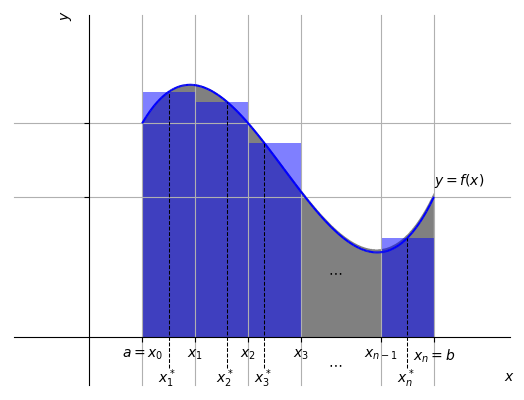
\includegraphics[width=0.9\textwidth]{./cap_int/dados/fig_soma_de_Riemann/fig_soma_de_Riemann}
  \caption{Ilustração da soma de Riemann.}
  \label{fig:soma_de_Riemann}
\end{figure}

\begin{obs}\normalfont{(Aproximação da área sob o gráfico)}
No caso de uma função não negativa, uma soma de Riemann é uma aproximação da área sob seu gráfico e o eixo das abscissas\footnote{Veja o Exercício \ref{exer:int_geoRiemann} para uma interpretação geométrica no caso geral de funções contínuas.}. Veja a Figura \ref{fig:soma_de_Riemann}.
\end{obs}

\subsection{Integral}

\begin{flushright}
  [Vídeo] | [Áudio] | \href{https://phkonzen.github.io/notas/contato.html}{[Contatar]}
\end{flushright}

A integral (definida) de $a$ até $b$ de uma dada função $f$ em relação a $x$ é denotada e definida por
\begin{equation}
  \int_a^b f(x)\,dx := \lim_{\|P\|\to 0} \sum_{i=1}^n f(x_i^*)\Delta x_i.
\end{equation}
De forma genérica, a integral definida de $a$ até $b$ é o limite das somas de Riemann quando a norma das partições $P$ do intervalo $[a, b]$ tendem a zero. Quando o limite existe, dizemos que $f$ é \emph{integrável} no intervalo $[a, b]$.

\begin{obs}
  Na notação de integral definida acima, chamamos $a$ de \emph{limite inferior} e $b$ de \emph{limite superior de integração}, $f$ é chamada de \emph{integrando} e $x$ de \emph{variável de integração}.
\end{obs}

\begin{obs}
  Funções contínuas são funções integráveis.
\end{obs}

\begin{figure}[H]
  \centering
  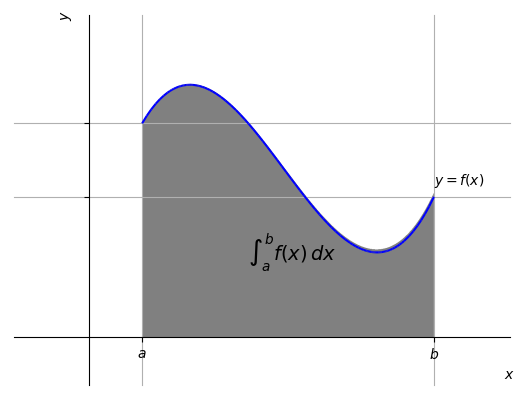
\includegraphics[width=0.9\textwidth]{./cap_int/dados/fig_geointdef/fig_geointdef}
  \caption{A integral definida como a área sob o gráfico.}
  \label{fig:geointdef}
\end{figure}

\begin{obs}\normalfont{(Área sob o gráfico)}\label{obs:int_area}
  No caso de uma função não negativa,
  \begin{equation}
    \int_a^b f(x)\,dx
  \end{equation}
  é a área sob o gráfico de $f$\footnote{Veja o Exercício \ref{exer:int_geointdef} para uma interpretação geométrica no caso geral de funções contínuas.}. Veja a Figura \ref{fig:geointdef}.  
\end{obs}

\begin{ex}
  Vamos calcular
  \begin{equation}
    \int_0^1 1\,dx.
  \end{equation}
  Aqui, o integrando é a função constante $f(x) \equiv 1$ e o \emph{intervalo de integração} é $[a, b]$. Da Observação \ref{obs:int_area}, temos que esta integral é a área sob o gráfico de $f$ no intervalo $[0, 1]$. Esta área é um retângulo de altura $1$ e comprimento $1$. Logo,
  \begin{equation}
    \int_0^1 1\,dx = 1\cdot 1 = 1.
  \end{equation}

  \ifispython
  Com o {\python}+{\sympy}, podemos computar esta integral com os seguintes comandos
  \begin{lstlisting}
    ...: from sympy import *
    ...: x = Symbol('x')
    ...: integrate(1, (x,0,1))
    Out: 1
  \end{lstlisting}
  \fi
\end{ex}

\subsection*{Exercícios resolvidos}

\begin{exeresol}
  Calcule
  \begin{equation}
    \int_{-1}^1 \sqrt{1 - x^2}\,dx.
  \end{equation}
\end{exeresol}
\begin{resol}
  Esta integral corresponde à área sob o gráfico da função $f(x) = \sqrt{1 - x^2}$ restrita ao intervalo $[-1, 1]$. Observando que
  \begin{align}
    y = \sqrt{x^2 - 1} &\Rightarrow y^2 = 1 - x^2\\
                       &\Rightarrow y^2 + x^2 = 1,
  \end{align}
  vemos que esta é a área do semicírculo de raio $1$. Logo,
  \begin{equation}
    \int_{-1}^1 \sqrt{1 - x^2}\,dx = \frac{\pi \cdot 1^2}{2} = \frac{\pi}{2}.
  \end{equation}

  \ifispython
  Com o {\python}+{\sympy}, podemos computar esta integral com os seguintes comandos
  \begin{lstlisting}
    In : from sympy import *
    ...: x = Symbol('x')
    ...: integrate(sqrt(1-x**2), (x,-1,1))
    Out: pi/2
  \end{lstlisting}
  \fi
\end{resol}

\begin{exeresol}
  Determine a função $F(x)$ tal que
  \begin{equation}
    F(x) = \int_0^x t\,dt,
  \end{equation}
  para todo $x\geq 0$. Então, mostre que $F'(x) = x$.
\end{exeresol}
\begin{resol}
  A integral definida
  \begin{equation}
    \int_0^x t\,dt
  \end{equation}
  é a área sob o gráfico de $f(t) = t$ restrita no intervalo $[0, x]$. Isto é, a área do triângulo retângulo de base $x$ e altura $x$. Logo,
  \begin{equation}
    F(x) = \int_0^x t\,dt = \frac{x\cdot x}{2} = \frac{x^2}{2}.
  \end{equation}
  Ou seja, temos $F(x) = x^2/2$ e, portanto,
  \begin{equation}
    F'(x) = \frac{1}{2}\cdot 2x = x.
  \end{equation}

  \ifispython
  Com o {\python}+{\sympy}, podemos fazer essas computações com os seguintes comandos
  \begin{lstlisting}
    In : from sympy import *
    ...: x, t = symbols('x,t')
    ...: F = integrate(t, (t,0,x))
    ...: print("F(x) = ", F)
    ...: 
    F(x) =  x**2/2
    In : diff(F,x)
    Out: x
  \end{lstlisting}
  \fi  
\end{resol}

\subsection*{Exercícios}

\begin{flushright}
  [Vídeo] | [Áudio] | \href{https://phkonzen.github.io/notas/contato.html}{[Contatar]}
\end{flushright}

\begin{exer}
  Calcule
  \begin{equation}
    \int_{-1}^2 2\,dx.
  \end{equation}
\end{exer}
\begin{resp}
  $6$
\end{resp}

\begin{exer}
  Calcule
  \begin{equation}
    \int_{-3}^{-1} 1-x\,dx.
  \end{equation}
\end{exer}
\begin{resp}
  $6$
\end{resp}

\begin{exer}
  Determine $F(x)$ tal que
  \begin{equation}
    F(x) = \int_{0}^{x} t+1\,dt.
  \end{equation}
  para $x\geq 0$. Então, calcule $F'(x)$.
\end{exer}
\begin{resp}
  $\displaystyle F(x) = \frac{x^2}{2} + x$; $F'(x) = x + 1$.
\end{resp}

\begin{exer}\label{exer:int_geoRiemann}
  Faça uma interpretação geométrica da uma soma de Riemann aplicada a uma função contínua e não positiva. Estenda sua interpretação para funções contínuas arbitrárias.
\end{exer}
\begin{resp}
  Dica: a soma de Riemann é uma aproximação da área líquida sob o gráfico da função.
\end{resp}

\begin{exer}\label{exer:int_geointdef}
  Faça uma interpretação geométrica de
  \begin{equation}
    \int_a^b f(x)\,dx
  \end{equation}
  quando $f$ é uma função contínua e não positiva. Estenda sua interpretação para funções contínuas arbitrárias.
\end{exer}
\begin{resp}
  Dica: $\displaystyle \int_a^b f(x)\,dx$é a área líquida sob o gráfico da função.
\end{resp}

\begin{exer}
  Calcule
  \begin{equation}
    \int_{-1}^2 -1\,dx.
  \end{equation}
\end{exer}
\begin{resp}
  $-3$
\end{resp}

\begin{exer}
  Calcule
  \begin{equation}
    \int_{-1}^{1} x\,dx.
  \end{equation}
\end{exer}
\begin{resp}
  $0$
\end{resp}

\section{Propriedades de integração}\label{cap_int_sec_propint}

\begin{flushright}
  [Vídeo] | [Áudio] | \href{https://phkonzen.github.io/notas/contato.html}{[Contatar]}
\end{flushright}

Na Seção \ref{cap_int_sec_nocaoint}, vimos que a integral definida de uma dada função $f$ em um intervalo $[a, b]$ está associada à área (líquida) entre seu gráfico e as retas $y=0$, $x=a$ e $x=b$. Veja a Figura \ref{fig:geointdef}.

Com base nesta noção geométrica, podemos inferir as seguintes propriedades de integração para funções integráveis $f$ e $g$:
\begin{enumerate}[a)]
\item $\displaystyle \int_a^a f(x)\,dx = 0$
\item $\displaystyle \int_a^b k\cdot f(x)\,dx = k\cdot\int_a^b f(x)\,dx$
\item $\displaystyle \int_a^b \left[f(x)\pm g(x)\right]\,dx = \int_a^b f(x)\,dx \pm \int_a^b g(x)\,dx$
\item $\displaystyle \int_a^b f(x)\,dx = \int_a^c f(x)\,dx + \int_c^b f(x)\,dx$
\item $\displaystyle \min_{x\in [a, b]} \{f(x)\}\cdot (b-a) \leq \int_a^b f(x)\,dx \leq \max_{x\in [a, b]} \{f(x)\}\cdot (b-a)$
\end{enumerate}

\begin{ex}
  Sejam $f$ e $g$ funções integráveis tais que
  \begin{align}
    \int_{-1}^4 f(x)\,dx = 2,\\
    \int_4^5 f(x)\,dx = 3,\\
    \int_{-1}^4 g(x)\,dx = -1.
  \end{align}
  Então, vejamos os seguintes casos:
  \begin{enumerate}[a)]
  \item
    \begin{equation}
      \int_{4}^{-1} g(x)\,dx = -\int_{-1}^4 g(x)\,dx = -(-1) = 1.
    \end{equation}
  \item
    \begin{equation}
      \int_{-1}^{-1} 4f(x)\,dx = 0.
    \end{equation}
  \item
    \begin{equation}
      \int_{-1}^{4} -2g(x)\,dx = -2\int_{-1}^4 g(x)\,dx = 2.
    \end{equation}
  \item
    \begin{align}
      \int_{-1}^{4} \left[f(x) - 2g(x)\right]\,dx &= \int_{-1}^{4} f(x)\,dx - \int_{-1}^4 2g(x)\,dx \\
                                                  &= 2 - 2\int_{-1}^4 g(x)\,dx \\
                                                  &= 2 + 2 = 4.
    \end{align}
  \item
    \begin{align}
      \int_{-1}^5 f(x)\,dx &= \int_{-1}^4 f(x)\,dx + \int_{4}^5 f(x)\,dx \\
                           &= 2 + 3 = 5.
    \end{align}
  \end{enumerate}
\end{ex}

\begin{ex}
  Lembrando que $-1 \leq \sen x \leq 1$, temos da propriedade e) acima que
  \begin{align}
    &2\pi \min_{x\in [-\pi, \pi]} \{\sen(x)\} \leq \int_{-\pi}^\pi \sen(x)\,dx \leq 2\pi \max_{x\in [\-pi, \pi]} \{\sen(x)\} \\
    &\Rightarrow -2\pi \leq \int_{-\pi}^\pi \sen(x)\,dx \leq 2\pi.
  \end{align}
\end{ex}

\subsection{Teorema do valor médio}

\begin{flushright}
  [Vídeo] | [Áudio] | \href{https://phkonzen.github.io/notas/contato.html}{[Contatar]}
\end{flushright}

Com base na noção de integral, define-se a média de uma função $f$ no intervalo $[a, b]$ por
\begin{equation}
  \frac{1}{b-a}\int_a^b f(x)\,dx,
\end{equation}
no caso de $f$ ser integrável neste intervalo.

\begin{teo}\normalfont{(Teorema do valor médio para integrais)}\label{teo:int_teomed}
  Se $f$ for contínua em $[a, b]$, então existe $c\in [a, b]$ tal que
  \begin{equation}
    f(c) = \frac{1}{b-a}\int_a^b f(x)\,dx.
  \end{equation}
\end{teo}
\begin{dem}
  Vejamos uma ideia da demonstração. Da propriedade de integração e) acima, temos
  \begin{equation}
    \min_{x\in [a, b]} \{f(x)\} \leq \frac{1}{b-a}\int_a^b f(x)\,dx \leq \max_{x\in [a, b]} \{f(x)\}.
  \end{equation}
  Agora, pelo Teorema do valor intermediário (Teorema \ref{teo:valorintermediario}), temos $f$ assume todos os valores entre seus valores mínimo e máximo. Logo, existe $c\in [a, b]$ tal que
  \begin{equation}
    f(c) = \frac{1}{b-a}\int_a^b f(x)\,dx.
  \end{equation}  
\end{dem}

\begin{ex}
  Seja $f$ uma função contínua em $[a, b]$, $a\neq b$, e
  \begin{equation}
    \int_a^b f(x)\,dx = 0,
  \end{equation}
  então $f$ possui pelo menos um zero neste intervalo. De fato, do Teorema do valor médio para integrais, temos que existe $c\in [a, b]$ tal que
  \begin{equation}
    f(c) = \frac{1}{b-a}\int_a^b f(x)\,dx = \frac{1}{b-a}\cdot 0 = 0.
  \end{equation}
\end{ex}

\subsection{Teorema fundamental do cálculo, parte I}

\begin{flushright}
  [Vídeo] | [Áudio] | \href{https://phkonzen.github.io/notas/contato.html}{[Contatar]}
\end{flushright}

Seja $f$ uma função integrável e $F$ a função definida por
\begin{equation}
  F(x) = \int_a^x f(t)\,dt,
\end{equation}
para algum número real $a$ dado.

\begin{teo}\normalfont{(Teorema fundamental do cálculo, parte I)}\label{teo:int_tfc1}
  Se $f$ é contínua em $[a, b]$, então é contínua em $[a, b]$ e diferenciável em $(a, b)$ a função
  \begin{equation}
    F(x) = \int_a^x f(t)\,dt
  \end{equation}
  sendo
  \begin{equation}
    F'(x) = \frac{d}{dx}\int_a^x f(t)\,dt = f(x).
  \end{equation}
\end{teo}
\begin{dem}
  Vejamos a ideia da demonstração. Da definição de derivada, temos
  \begin{align}
    F'(x) &= \lim_{h\to 0} \frac{F(x+h) - F(x)}{h} \\
          &= \lim_{h\to 0} \frac{1}{h}\left[\int_a^{x+h} f(x)\,dx - \int_a^x f(x)\, dx\right] \\
          &= \lim_{h\to 0} \frac{1}{h}\int_x^{x+h} f(x)\,dx.
  \end{align}
  Agora, do Teorema do valor médio para integrais (Teorema \ref{teo:int_teomed}), temos que existe $c_h \in [x, x+h]$ tal que
  \begin{align}
    f(c_h) &= \frac{1}{x+h-x}\int_x^{x+h} f(x)\,dx \\
           &= \frac{1}{h}\int_x^{x+h} f(x)\,dx.
  \end{align}
  Notemos que $c_h\to x$ quando $h\to 0$ e, portanto, temos
  \begin{align}
    F'(x) &= \lim_{h\to 0} \frac{1}{h}\int_x^{x+h} f(x)\,dx \\
          &= \lim_{h\to 0} f(c_h) \\
          &= f(x).
  \end{align}
\end{dem}

\begin{ex}
  Vejamos os seguintes casos:
  \begin{enumerate}[a)]
  \item
    \begin{equation}
      \frac{d}{dx}\int_1^x t^2\,dt = x^2.
    \end{equation}
  \item
    \begin{equation}
      \frac{d}{dx}\int_0^x \sen(t)\,dt = \sen(x)
    \end{equation}
  \end{enumerate}

  \ifispython
  Com o {\python}+{\sympy}, podemos computar os resultados acima com os seguintes comandos:
  \begin{lstlisting}
    In : from sympy import *
    ...: x, t = symbols('x,t')
    ...: # a)
    ...: diff(integrate(t**2, (t,1,x)))
    ...: 
    Out: x**2
    
    In : diff(integrate(sin(t), (t,0,x)))
    Out: sin(x)
  \end{lstlisting}
  \fi
\end{ex}

\subsection{Integral indefinida}

\begin{flushright}
  [Vídeo] | [Áudio] | \href{https://phkonzen.github.io/notas/contato.html}{[Contatar]}
\end{flushright}

A parte I do Teorema fundamental do cálculo (Teorema \ref{teo:int_tfc1}), mostra que a derivada da integral de uma função $f$ (contínua) é uma função $F$ tal que
\begin{equation}
  F'(x) = f(x).
\end{equation}
Dizemos que $F$ é uma \emph{primitiva} da função $f$.

Observamos que se $F$ é uma primitiva de $f$, então $G(x) = F(x) + C$ também é primitiva de $f$ para qualquer constante $C$, i.e.
\begin{align}
  G'(x) &= (F(x) + C)' \\
        &= F'(x) + (C)' \\
        &= f(x) + 0 \\
        &= f(x).
\end{align}
Mais ainda, do Corolário \ref{corol:apderiv_teomed_2} do Teorema do valor médio para derivadas, temos que quaisquer duas primitivas de uma mesma função diferem-se apenas uma constante.

Com isso, definimos a \emph{integral indefinida} de $f$ em relação a $x$ por
\begin{equation}
  \int f(x)\,dx = F(x) + C,
\end{equation}
onde $F$ é qualquer primitiva de $f$ e $C$ uma constante indeterminada.

\begin{ex}
  Vejamos os seguintes casos:
  \begin{enumerate}[a)]
  \item $\displaystyle \int \,dx = x + C$
  \item $\displaystyle \int 2x\,dx = x^2 + C$
  \item $\displaystyle \int \cos(x)\,dx = \sen(x) + C$
  \item $\displaystyle \int e^x\,dx = e^x + C$
  \end{enumerate}
  \ifispython
  Com o {\python}+{\sympy}, podemos computar as integrais indefinidas acima com os seguintes comandos:
  \begin{lstlisting}
    In : from sympy import *
    In : x = symbols('x')
    ...: # a)
    ...: integrate(1, x)
    ...: 
    Out: x
    # b)
    In : integrate(2*x, x)
    ...: 
    Out: x**2
    # c)
    In : integrate(cos(x), x)
    ...: 
    Out: sin(x)
    # d)
    In : integrate(exp(x), x)
    Out: exp(x)
  \end{lstlisting}
  \fi  
\end{ex}

\subsection{Teorema fundamental do cálculo, parte II}

\begin{flushright}
  [Vídeo] | [Áudio] | \href{https://phkonzen.github.io/notas/contato.html}{[Contatar]}
\end{flushright}

\begin{teo}\normalfont{(Teorema fundamental do cálculo, parte II)}\label{teo:int_tfc2}
  Se $f$ é contínua em $[a, b]$ e $F$ é qualquer primitiva de $f$, então
  \begin{equation}
    \int_a^b f(x)\,dx = F(b) - F(a).
  \end{equation}
\end{teo}
\begin{dem}
  Vejamos a ideia da demonstração. A parte I do Teorema fundamental do cálculo (Teorema \ref{teo:int_tfc1}), nos garante a existência de
  \begin{equation}
    G(x) = \int_a^x f(t)\,dt.
  \end{equation}
  Seja, então, $F$ uma primitiva qualquer de $f$. Logo,
  \begin{align}
    F(b) - F(a) &= [G(b) + C] - [G(a) + C] \\
                &= G(b) - G(a) \\
                &= \int_a^b f(t)\,dx - \int_a^a f(t)\,dt \\
                &= \int_a^b f(t)\,dx.
  \end{align}
\end{dem}

\begin{ex}
  Vejamos os seguintes casos:
  \begin{enumerate}[a)]
  \item $\displaystyle \int_0^1 \,dx = \left. x \right|_0^1 = 1 - 0 = 1$
  \item $\displaystyle \int_0^1 x\,dx = \left.\frac{x^2}{2}\right|_0^1 = \frac{1^2}{2}-\frac{0^2}{2} = \frac{1}{2}$
  \item $\displaystyle \int_{-\frac{\pi}{2}}^{\frac{\pi}{2}} \cos(x)\,dx = \left.\sen(x)\right|_{-\frac{\pi}{2}}^{\frac{\pi}{2}} = \sen\left(\frac{\pi}{2}\right) - \sen\left(-\frac{\pi}{2}\right) = 2$
  \end{enumerate}
  \ifispython
  Com o {\python}+{\sympy}, podemos computar as integrais indefinidas acima com os seguintes comandos:
  \begin{lstlisting}
    In : from sympy import *
    ...: x = symbols('x')
    ...: # a)
    ...: integrate(1, (x,0,1))
    Out: 1
    ..: # b)
    In : integrate(x, (x,0,1))
    Out: 1/2
    ..: c)
    In : integrate(cos(x), (x,-pi/2,pi/2))
    Out: 2
  \end{lstlisting}
  \fi  
\end{ex}

\begin{obs}
  Do Teorema fundamental do cálculo, parte II, temos
  \begin{equation}
    \int_a^b f(x)\,dx = - \int_b^a f(x)\,dx.
  \end{equation}
  De fato, se $F$ é uma primitiva de $f$, então
  \begin{align}
    \int_a^b f(x)\,dx &= F(b) - F(a) \\
                      &= - \left[F(a) - F(b)\right] \\
                      &= - \int_b^a f(x)\,dx.
  \end{align}
\end{obs}

\begin{ex}
  Temos que
  \begin{equation}
    \int_0^1 dx = \left. x\right|_0^1 = 1 - 0 = 1.
  \end{equation}
  Agora,
  \begin{equation}
    \int_1^0 dx = \left. x\right|_1^0 = 0 - 1 = -1.
  \end{equation}
  Conforme esperado, temos
  \begin{equation}
    \int_0^1 dx = - \int_1^0 dx.
  \end{equation}
\end{ex}

\subsection*{Exercícios resolvidos}

\begin{flushright}
  [Vídeo] | [Áudio] | \href{https://phkonzen.github.io/notas/contato.html}{[Contatar]}
\end{flushright}

\begin{exeresol}
  Calcule
  \begin{equation}
    \int_1^{\sqrt{e}} x - \frac{1}{x}\,dx.
  \end{equation}
\end{exeresol}
\begin{resol}
  Primeiramente, notemos que
  \begin{align}
    & \int x\,dx = \frac{x^2}{2} + C,\\
    & \int \frac{1}{x}\,dx = \ln x + C.
  \end{align}
  Então, usando as propriedades de integração, temos
  \begin{align}
    \int_1^{\sqrt{e}} x - \frac{1}{x}\,dx &= \int_1^{\sqrt{e}} x\,dx - \int_1^{\sqrt{e}} \frac{1}{x}\,dx \\
                                 &= \left[\frac{x^2}{2}\right]_1^{\sqrt{e}} - \left[\ln x\right]_1^{\sqrt{e}} \\
                                          &= \left[\frac{(\sqrt{e})^2}{2} - \frac{1}{2}\right] - \left[\ln\sqrt{e} - \ln 1\right]\\
                                          &= \frac{e}{2} - \frac{1}{2} - \frac{1}{2}\ln(e) - 0 \\
                                          &= \frac{e}{2} - 1.
  \end{align}
  \ifispython
  Com o {\python}+{\sympy}, podemos computar essa integral definida com os seguintes comandos:
  \begin{lstlisting}
    In : from sympy import *
    ...: x = symbols('x')
    ...: integrate((x - 1/x), (x,1,sqrt(E)))
    Out: -1 + E/2
  \end{lstlisting}
  \fi  
\end{resol}

\begin{exeresol}
  Calcule a área entre o gráfico de $f(x) = \sen(x)$ e as retas $y=0$, $x=-\pi/2$ e $x=\pi/2$.
\end{exeresol}
\begin{resol}
  Lembrando que a integral definida está associada a área sob o gráfico do integrando, temos que a área desejada pode ser calculada por
  \begin{equation}
    A = - \int_{-\frac{\pi}{2}}^0 \sen(x)\,dx + \int_0^{\frac{\pi}{2}} \sen(x)\,dx,
  \end{equation}
  pois $\sen(x) < 0$ para $x\in (-\pi/2, 0)$ e $\sen(x) > 0$ para $x\in (0, \pi/2)$.
  Também, observamos que
  \begin{equation}
    \int \sen(x)\,dx = -\cos(x) + C.
  \end{equation}
  Logo, do Teorema fundamental do cálculo segue que
  \begin{align}
    A &= - \int_{-\frac{\pi}{2}}^0 \sen(x)\,dx + \int_0^{\frac{\pi}{2}} \sen(x)\,dx \\
      &= -\left[-\cos(x)\right]_{-\frac{\pi}{2}}^0 + \left[-\cos(x)\right]_0^{\frac{\pi}{2}} \\
      &= -[-1 - 0] + [-0 - (-1)] = 2. 
  \end{align}
  \ifispython
  Com o {\python}+{\sympy}, podemos computar essa integral definida com os seguintes comandos:
  \begin{lstlisting}
    In : from sympy import *
    ...: x = symbols('x')
    ...: A = -integrate(sin(x), (x,-pi/2,0))
    ...: A += integrate(sin(x), (x,0,pi/2))
    ...: A
    Out: 2
  \end{lstlisting}
  \fi  
\end{resol}

\begin{exeresol}
  Encontre a função $y = y(x)$ tal que
  \begin{equation}
    \frac{dy}{dx} = x,
  \end{equation}
  e $y(0) = 1$.
\end{exeresol}
\begin{resol}
  Integrando ambos os lados da equação diferencial em relação a $x$, temos
  \begin{gather}
    \int \frac{dy}{dx}\,dx = \int x\,dx \\
    y = \frac{x^2}{2} + C \\
  \end{gather}
  Agora, da condição $y(0) = 1$, segue
  \begin{gather}
    y(0) = 1 \\
    \frac{0^2}{2} + C = 1 \\
    C = 1.
  \end{gather}
  Concluímos que $y = x^2/2 + 1$.
  \ifispython
  Com o {\python}+{\sympy}, podemos resolver esta computar essa integral definida com os seguintes comandos:
  \begin{lstlisting}
    In : from sympy import *
    ...: y = Function('y')
    ...: x = symbols('x')
    ...: dsolve(Eq(diff(y(x),x), x), y(x), ics={y(0):1})
    Out: Eq(y(x), x**2/2 + 1)
  \end{lstlisting}
  \fi  
\end{resol}

\subsection*{Exercícios}

\begin{flushright}
  [Vídeo] | [Áudio] | \href{https://phkonzen.github.io/notas/contato.html}{[Contatar]}
\end{flushright}

\begin{exer}
  Sejam $f$ e $g$ tais que
  \begin{align}
    &\int_{-2}^{0} f(x)\,dx = -2,\quad\int_{-1}^{0} f(x)\,dx = \frac{1}{2},\\
    &\int_{-2}^0 g(x)\,dx = 1.
  \end{align}
  Calcule
  \begin{enumerate}[a)]
  \item $\displaystyle \int_{-1}^{-1} f(x) - 51\cdot g(x)\,dx$
  \item $\displaystyle \int_{-2}^{0} 2g(x) - \frac{1}{2}f(x)\,dx$
  \item $\displaystyle \int_{-2}^{-1} f(x)\,dx$
  \end{enumerate}
\end{exer}
\begin{resp}
  a)~$0$; b)~$3$; c)~$-5/2$
\end{resp}

\begin{exer}
  Calcule
  \begin{enumerate}[a)]
  \item $\displaystyle\int_{-1}^2 2\,dx$
  \item $\displaystyle\int_{-3}^{-1} 1-x\,dx$
  \item $\displaystyle\int_{1}^{e} \frac{2}{x}\,dx$
  \end{enumerate}
\end{exer}
\begin{resp}
  a)~$6$; b)~$6$; c)~$2$
\end{resp}

\begin{exer}
  Calcule a área entre o gráfico de $f(x) = x^2-1$ e as retas $y=0$, $x=0$ e $x=2$.
\end{exer}
\begin{resp}
  $4/3$
\end{resp}

\begin{exer}
  Encontre a função $y = y(x)$ tal que
  \begin{equation}
    \frac{dy}{dx} = \cos(x),
  \end{equation}
  e $y(\pi) = 1$.
\end{exer}
\begin{resp}
  $y = \sen(x) + 1$
\end{resp}

\section{Regras básicas de integração}\label{cap_int_sec_regrasbasic}

\begin{flushright}
  [Vídeo] | [Áudio] | \href{https://phkonzen.github.io/notas/contato.html}{[Contatar]}
\end{flushright}

Na Seção \ref{cap_int_sec_propint}, definimos a integral indefinida por
\begin{equation}
  \int f(x)\,dx = F(x) + C,
\end{equation}
onde $F$ é uma \emph{primitiva} de $f$, i.e. $F' = f$, e $C$ é uma \emph{constante indeterminada}. Na sequência, vamos discutir sobre as regras básicas para o cálculo de integrais.

\subsection{Integral de função potência}

\begin{flushright}
  [Vídeo] | [Áudio] | \href{https://phkonzen.github.io/notas/contato.html}{[Contatar]}
\end{flushright}

Com base na derivada de função potência, podemos afirmar que
\begin{equation}
  {\color{blue}\int x^r\,dx = \frac{x^{r+1}}{r+1} + C,\quad r\neq -1}.
\end{equation}
De fato, temos
\begin{align}
  F(x) &= \frac{x^{r+1}}{r+1} + C \\
  F'(x) &= (r+1) \frac{x^r}{r+1} \\
  &= x^r,
\end{align}
para $r\neq -1$.

\begin{ex}
  Estudamos os seguintes casos:
  \begin{enumerate}[a)]
  \item
    \begin{equation}
      \int x\,dx = \frac{x^2}{2} + C.
    \end{equation}
  \item
    \begin{align}
      \int \frac{1}{x^2}\,dx &= \int x^{-2}\,dx \\
                             &= -x^{-1} + C \\
                             &= -\frac{1}{x}+C.
    \end{align}
    \ifispython
    Verifique com o {\python}+{\sympy}!
    \fi
  \end{enumerate}
\end{ex}

\begin{ex}
  Vamos calcular
  \begin{equation}
    \int_{-1}^1 x^2\,dx.
  \end{equation}
  Da regra da potência, temos
  \begin{equation}
    \int x^2\,dx = \frac{x^3}{3} + C.
  \end{equation}
  Logo, do Teorema Fundamental do Cálculo, temos
  \begin{align}
    \int_{-1}^1 x^2\,dx &= \left.\frac{x^3}{3}\right|_{-1}^1 \\
                        &= \frac{1^3}{3} - \frac{(-1)^3}{3} \\
                        &= \frac{1}{3} + \frac{1}{3} = \frac{2}{3}.
  \end{align}
    \ifispython
    Verifique com o {\python}+{\sympy}!
    \fi
\end{ex}

\subsection{Regra da multiplicação por constante}

\begin{flushright}
  [Vídeo] | [Áudio] | \href{https://phkonzen.github.io/notas/contato.html}{[Contatar]}
\end{flushright}

Seja $k$ uma constante. Então, temos a seguinte regra da multiplicação por constante
\begin{equation}
  {\color{blue}\int k\cdot f(x)\,dx = k\cdot \int f(x)\,dx}
\end{equation}
De fato, se $F$ uma primitiva de $f$, então pela regra da multiplicação por constante para derivadas, temos
\begin{align}
  (k\cdot F)' &= k\cdot F'\\
              &= k\cdot f,
\end{align}
i.e. $k\cdot F$ é primitiva de $k\cdot f$.

\begin{ex}
  Estudamos os seguintes casos:
  \begin{enumerate}[a)]
  \item
    \begin{align}
      \int 2x\,dx &= 2\int x\,dx\\
                  &= 2\left(\frac{x^2}{2} + C\right)\\
                  &= x^2 + 2C\\
                  &= x^2 + C
    \end{align}
    Aqui, fizemos um abuso de linguagem ao assumir $2C = C$. Isso pode ser feito, pois $C$ denota uma constante indeterminada e, multiplicá-la por dois continua sendo indeterminada e constante. Vamos fazer este tipo de simplificação de notação várias vezes ao longo do texto.
  \item
    \begin{align}
      \int \frac{1}{3}\sqrt{x}\,dx &= \frac{1}{3}\int x^{\frac{1}{2}}\,dx\\
                                   &= \frac{1}{3}\frac{x^{\frac{1}{2}+1}}{\frac{1}{2}+1} + C\\
                                   &= \frac{1}{3}\frac{x^{\frac{3}{2}}}{\frac{3}{2}} + C\\
                                   &= \frac{2}{9}\sqrt{x^3} + C
    \end{align}
  \item
    \begin{align}
      \int_0^{1}-x^2\,dx &= -\int_0^1x^2\,dx\\
                         &= \int_1^0 x^2\,dx\\
                         &= \left.\frac{x^3}{3}\right|_1^0\\
                         &= \frac{0^3}{3} - \frac{1^3}{3}\\
                         &= \frac{1}{3}
    \end{align}
    \ifispython
    Verifique com o {\python}+{\sympy}!
    \fi
  \end{enumerate}
\end{ex}

\subsection{Regra da soma ou subtração}

Se $f$ e $g$ são funções integráveis, então vale a seguinte regra da soma/subtração
\begin{equation}
  {\color{blue}\int \left[f(x)\pm g(x)\right]\,dx = \int f(x)\,dx \pm \int g(x)\,dx}.
\end{equation}
De fato, sejam $F$ uma primitiva de $f$ e $G$ uma primitiva de $g$. Temos
\begin{align}
  (F \pm G)' &= F' \pm G'\\
             &= f \pm g,
\end{align}
i.e. $F \pm G$ é primitiva de $f+g$.

\begin{ex}
  Estudamos os seguintes casos:
  \begin{enumerate}[a)]
  \item
    \begin{align}
      \int x + 1\,dx &= {\color{blue}\int x\,dx} + {\color{red}\int\,dx}\\
                     &= {\color{blue}\frac{x^2}{2} + C_1} + {\color{red}x + C_2}\\
                     &= \frac{x^2}{2} + x + C
    \end{align}
    Aqui, $C_1$, $C_2$ e $C = C_1+C_2$ denotam constantes indeterminadas.
  \item
    \begin{align}
      \int \sqrt{x} - x\,dx &= {\color{blue}\int x^{\frac{1}{2}}\,dx} - {\color{red}\int x\,dx}\\
                            &= {\color{blue}\frac{3}{2}x^{\frac{3}{2}}} - {\color{red}\frac{x^2}{2}} + C
    \end{align}
  \item
    \begin{align}
      {\color{blue}\int (2x^2 + 3x - 1)\,dx} &= \int \left[2x^2 + (3x - 1)\right]\,dx\\
                                             &= \int 2x^2\,dx + \int 3x - 1 \,dx \\
                                             &= {\color{blue}\int 2x^2\,dx - \int 3x\,dx - \int \,dx}\\
                                             &= 2\int x^2\,dx + 3\int x\,dx - \int \,dx\\
                                             &= \frac{2}{3}x^3 + \frac{3}{2}x^2 - x + C
    \end{align}
  \end{enumerate}
\end{ex}

\begin{ex}
  Vamos calcular
  \begin{equation}
    \int_{0}^1 x^2 + 1\,dx.
  \end{equation}
  Temos
  \begin{align}
    \int x^2 + 1\,dx &= \int x^2\,dx + \int \,dx\\
                     &= \frac{x^3}{3} + x + C.
  \end{align}
  Agora, do Teorema Fundamental do Cálculo, temos
  \begin{align}
    \int_0^1 x^2+1\,dx &= \left. \frac{x^3}{3} + x\right|_0^1 \\
                       &= \frac{1}{3} + 1 - \left(\frac{0^3}{3} + 0\right) \\
                       &= \frac{4}{3}.
  \end{align}
\end{ex}

\subsection{Integral de $x^{-1}$}

\begin{flushright}
  [Vídeo] | [Áudio] | \href{https://phkonzen.github.io/notas/contato.html}{[Contatar]}
\end{flushright}

Começamos lembrando que, para $x>0$, temos
\begin{equation}
  \frac{d}{dx}\ln x = \frac{1}{x}
\end{equation}
Agora, pela regra da cadeia, para $x<0$, temos
\begin{align}
  \frac{d}{dx}\ln(-x) &= \frac{1}{-x}\cdot (-x)'\\
                      &= -\frac{1}{x}\cdot (-1)\\
                      &= \frac{1}{x}
\end{align}
Ou seja, temos que
\begin{equation}
  \frac{d}{dx}\ln|x| = \frac{1}{x}
\end{equation}
donde, concluímos que
\begin{equation}
  {\color{blue}\int\frac{1}{x}\,dx = \ln|x| + C}
\end{equation}

\begin{ex}
  Vamos calcular
  \begin{equation}
    \int_1^e x^{-1}\,dx.
  \end{equation}
  Usando o Teorema Fundamental do Cálculo, temos
  \begin{align}
    \int_1^e x^{-1}\,dx &= \int_1^e \frac{1}{x}\,dx\\
                        &= \left. \ln|x|\right|_1^e \\
                             &= \ln|e| - \ln|1| \\
                             &= 1 - 0 = 1.
  \end{align}
  \ifispython
  Verifique computando com o {\python}+{\sympy}!
  \fi
\end{ex}

\subsection{Integral da função exponencial natural}\label{cap_int_subsec_funexp}

\begin{flushright}
  [Vídeo] | [Áudio] | \href{https://phkonzen.github.io/notas/contato.html}{[Contatar]}
\end{flushright}

Da derivada da função exponencial natural, temos
\begin{equation}
  {\color{blue}\int e^x\,dx = e^x + C}.
\end{equation}

\begin{ex}
  Vamos estudar os seguintes casos:
  \begin{enumerate}[a)]
  \item
    \begin{align}
      \int e^{2 + x}\,dx &= \int e^2e^x\,dx \\
                         &= e^2\int e^x\,dx \\
                         &= e^2e^x + C \\
                         &= e^{2+x} + C
    \end{align}
  \item
    \begin{align}
      \int_{0}^{\ln 2}e^x\,dx &= \left. e^x\right|_0^{\ln 2}\\
                              &= e^{\ln 2} - e^0\\
                              &= 2 - 1\\
                              &= 1
    \end{align}
\end{enumerate}
\end{ex}

\subsection{Integrais de funções trigonométricas}\label{cap_int_sec_regrasbasic_trigo}

\begin{flushright}
  [Vídeo] | [Áudio] | \href{https://phkonzen.github.io/notas/contato.html}{[Contatar]}
\end{flushright}

Com base na derivada de funções trigonométricas, temos
\begin{itemize}
\item
  \begin{equation}
    \pmb{\int \sen(x)\,dx = -\cos(x) + C}
  \end{equation}
\item
  \begin{equation}
    \pmb{\int \cos(x)\,dx = \sen(x) + C}
  \end{equation}
\end{itemize}

\begin{ex}
  Vamos calcular
  \begin{equation}
    \int_0^{\pi} \cos(x) - \sen(x)\,dx.
  \end{equation}
  Temos
  \begin{align}
    \int \cos(x)-\sen(x)\,dx &= \int\cos(x)\,dx - \int\sen(x)\,dx\\
                             &= \sen(x) + \cos(x) + C.
  \end{align}
  Agora, do Teorema Fundamental do Cálculo, obtemos
  \begin{align}
    \int_0^{\pi} \cos(x)-\sen(x)\,dx &= \left.\sen(x) + \cos(x)\right|_0^\pi \\
                             &= \sen(\pi)+\cos(\pi) - \left[\sen(0)+\cos(0)\right]\\
                             &= -1 - 1 = -2.
  \end{align}
\end{ex}


\subsection{Tabela de integrais}

\begin{flushright}
  [Vídeo] | [Áudio] | \href{https://phkonzen.github.io/notas/contato.html}{[Contatar]}
\end{flushright}

\begin{small}
\begin{align}
  & \int k\cdot f(x)\,dx = k\cdot\int f(x)\,dx\\
  & \int \left[f(x)\pm g(x)\right]\,dx = \int f(x)\,dx \pm \int g(x)\,dx\\
  & \int x^r\,dx = \frac{x^{r+1}}{r+1} + C,\quad r\neq -1\\
  & \int \frac{1}{x}\,dx = \ln x + C \\
  & \int e^x\,dx = e^x + C \\
  & \int \sen(x)\,dx = -\cos(x) + C \\
  & \int \cos(x)\,dx = \sen(x) + C
\end{align}
\end{small}

\subsection*{Exercícios resolvidos}

\begin{flushright}
  [Vídeo] | [Áudio] | \href{https://phkonzen.github.io/notas/contato.html}{[Contatar]}
\end{flushright}

\begin{exeresol}
  Calcule a área total entre as curvas $y=x^2-1$, $y=0$, $x=0$ e $x=2$.
\end{exeresol}
\begin{resol}
  Tendo em vista que $x^2-1\leq 0$ para $x\in [0, 1]$ e $x^2-1\geq [0, 1]$, temos que a área $A$ pedida é igual a
  \begin{equation}
    A = -\int_0^1 x^2 -1\,dx + \int_1^2 x^2-1\,dx.
  \end{equation}
  Agora, calculamos a seguinte integral indefinida
  \begin{align}
    \int x^2 - 1\,dx &= \int x^2\,dx - \int\,dx \\
                     &= \frac{x^3}{3} - x + C.
  \end{align}
  Então, usando o Teorema Fundamental do Cálculo, obtemos
  \begin{align}
    A &= -\left[\frac{x^3}{3}-x\right]_0^1 + \left[\frac{x^3}{3}-x\right]_1^2\\
      &= - \left[\frac{1}{3}-1\right] + \left[\frac{8}{3} - 2 - \frac{1}{3} + 1\right] \\
      &= \frac{2}{3} \frac{4}{3} = 2.
  \end{align}
\ifispython
Podemos usar o \sympy~para calcular a área, com os seguintes comandos\footnote{Veja a Observação \ref{obs:cap_int_python}.}:
\begin{verbatim}
>>> -integrate(x**2-1,(x,0,1))+integrate(x**2-1,(x,1,2))
2
\end{verbatim}
\fi  
\end{resol}

\begin{exeresol}
  Calcule
  \begin{equation}
    \int \frac{1}{2x}\,dx.
  \end{equation}
\end{exeresol}
\begin{resol}
  Das regras básicas de integração, temos
  \begin{align}
    \int \frac{1}{2x}\,dx &= \int \frac{1}{2}\cdot\frac{1}{x}\,dx \\
                          &= \frac{1}{2}\int\frac{1}{x}\,dx \\
                          &= \frac{1}{2}\ln(x) + C \\
                          &= \ln\sqrt{x} + C.
  \end{align}
\ifispython
No \sympy, temos\footnote{Veja a Observação \ref{obs:cap_int_python}.}:
\begin{verbatim}
>>> integrate(1/(2*x),x)
log(x)/2
\end{verbatim}
\fi    
\end{resol}


\subsection{Exercícios}

\begin{flushright}
  [Vídeo] | [Áudio] | \href{https://phkonzen.github.io/notas/contato.html}{[Contatar]}
\end{flushright}

\begin{exer}
  Calcule
  \begin{enumerate}[a)]
  \item $\displaystyle \int \,dx$
  \item $\displaystyle \int x^{-2}\,dx$
  \item $\displaystyle \int \sqrt{x}\,dx$
  \item $\displaystyle \int \frac{1}{\sqrt{x}}\,dx$
  \end{enumerate}
\end{exer}
\begin{resp}
  a)~$\displaystyle x + C$; b)~$\displaystyle -\frac{1}{x} + C$; c)~$\displaystyle \frac{2}{3}x^{3/2} + C$; d)~$\displaystyle 2x^{1/2} + C$
\end{resp}

\begin{exer}
  Calcule
  \begin{enumerate}[a)]
  \item $\displaystyle \int 1 + x^{-2}\,dx$
  \item $\displaystyle \int x - \frac{1}{x}\,dx$
  \end{enumerate}
\end{exer}
\begin{resp}
  a)~$\displaystyle x-\frac{1}{x}+C$; b)~$\displaystyle \frac{x^2}{2} - \ln|x| + C$
\end{resp}

\begin{exer}
  Calcule
  \begin{enumerate}[a)]
  \item $\displaystyle 2\cos(x)\,dx$
  \item $\displaystyle 1 - \sen(x)\,dx$
  \end{enumerate}
\end{exer}
\begin{resp}
  a)~$\displaystyle 2\sen(x) + C$; b)~$\displaystyle x + \cos(x) + C$
\end{resp}

\begin{exer}
  Calcule
  \begin{equation}
    \int_{-1}^1 x^3\,dx.
  \end{equation}
\end{exer}
\begin{resp}
  $0$
\end{resp}

\begin{exer}
  Calcule a área total entre as curvas $y=x^3$, $y=0$, $x=-1$ e $x=1$.
\end{exer}
\begin{resp}
  $1/2$
\end{resp}


\section{Integração por substituição}\label{cap_int_sec_subs}

\begin{flushright}
  [Vídeo] | [Áudio] | \href{https://phkonzen.github.io/notas/contato.html}{[Contatar]}
\end{flushright}

Seja $u = u(x)$. A regra de integração por substituição é
\begin{equation}
  \pmb{\int f(u(x))u'(x)\,dx = \int f(u)\,du}.
\end{equation}
De fato, se
\begin{equation}
  \int f(u)\,du = F(u) + C,
\end{equation}
então, da regra da cadeira (Seção \ref{cap_deriv_sec_cadeia}), temos
\begin{align}
  \frac{d}{dx}F(u(x)) &= F'(u(x))u'(x) \\
                      &= f(u(x))u'(x),
\end{align}
i.e. $F(u(x))$ é primitiva de $f(u(x))u'(x)$.

\begin{ex}
  Vejamos os seguintes casos:
  \begin{enumerate}[a)]
  \item $\displaystyle\int 2(2x+1)^2\,dx$.
    
    Tomamos $f(u) = u^2$ com $u(x) = 2x+1$, donde $u'(x) = 2$. Logo
    \begin{align}
      \int 2(2x+1)^2\,dx &= \int f(u(x))u'(x)\,dx \\
                         &= \int f(u)\,du \\
                         &= \int u^2\,du \\
                         &= \frac{u^3}{3} + C \\
                         &= \frac{(2x+1)^3}{3} + C.
    \end{align}
  \item $\displaystyle\int \pi\sen(\pi x)\,dx$.
    
    Tomando $f(u)=\sen(u)$, $u=\pi x$, temos $u'(x)=\pi$. Logo
    \begin{align}
      \int \pi\sen(\pi x)\,dx &= \int f(u(x))u'(x)\,dx \\
                              &= \int f(u)\,du \\
                              &= \int \sen(u)\,du \\
                              &= -\cos(u) + C \\
                              &= -\cos(\pi x) + C.
    \end{align}
  \end{enumerate}
\end{ex}

\begin{ex}
  Consideremos
  \begin{equation}
    \int (2x+1)^2\,dx.
  \end{equation}
  Substituindo
  \begin{equation}
    u = 2x+1
  \end{equation}
  temos
  \begin{equation}
    \frac{du}{dx} = 2 \Rightarrow dx = \frac{du}{2}.
  \end{equation}
  Portanto,
  \begin{align}
    \int (2x+1)^2\,dx &= \int u^2\,\frac{du}{2}\\
                     &= \frac{1}{2}\int u^2\,du\\
                     &= \frac{1}{2}\frac{u^{2+1}}{2+1} + C\\
                     &= \frac{u^3}{6} + C\\
                     &= \frac{1}{6}(2x+1)^3 + C.
  \end{align}
\end{ex}


\subsection{Integral de função exponencial}

\begin{flushright}
  [Vídeo] | [Áudio] | \href{https://phkonzen.github.io/notas/contato.html}{[Contatar]}
\end{flushright}

Na Subseção \ref{cap_int_subsec_funexp}, vimos que
\begin{equation}
  \int e^x\,dx = e^x + C
\end{equation}
Agora, com a regra da substituição, temos
\begin{align}
  \int a^x\,dx &= \int e^{\ln a^x}\,dx \\
               &= \int e^{x\ln a}\,dx,
\end{align}
com $a>0$ e $a\neq 1$. Tomando
\begin{equation}
  u = x\ln a \Rightarrow du = \ln(a)dx.
\end{equation}
Segue que
\begin{align}
  \int a^x\,dx &= \int e^u\frac{du}{\ln a} \\
               &= \frac{1}{\ln a}\int e^u\,du \\
               &= \frac{e^u}{\ln a} + C \\
               &= \frac{e^{x\ln a}}{\ln a} + C \\
               &= \frac{e^{\ln a^x}}{\ln a} + C \\
               &= \frac{a^x}{\ln a} + C.
\end{align}
Ou seja, concluímos que
\begin{equation}
  \pmb{\int a^x\,dx = \frac{a^x}{\ln a} + C}.
\end{equation}

\begin{ex}
  Vamos calcular
  \begin{equation}
    \int x\cdot 2^{x^2}\,dx.
  \end{equation}
  Por substituição, tomamos
  \begin{equation}
    u = x^2 \Rightarrow du = 2xdx,
  \end{equation}
  segue
  \begin{align}
    \int x\cdot 2^{x^2}\,dx &= \int \cdot 2^{u}\frac{du}{2} \\
                            &= \frac{1}{2}\int \cdot 2^{u}\,du \\
                            &= \frac{1}{2}\frac{2^u}{\ln 2} + C \\
                            &= \frac{1}{2}\frac{2^{x^2}}{\ln 2} + C
  \end{align}
\end{ex}

\subsection{Integral de funções trigonométricas}

\begin{flushright}
  [Vídeo] | [Áudio] | \href{https://phkonzen.github.io/notas/contato.html}{[Contatar]}
\end{flushright}

Na Seção \ref{cap_int_sec_regrasbasic_trigo}, vimos que
\begin{align}
  &\int \sen(x)\,dx = -\cos(x) + C \quad\text{e}\\
  &\int \cos(x)\,dx = \sen(x) + C.
\end{align}

\begin{ex}
  Vamos calcular
  \begin{equation}
    \int \sen^2(x)\,dx.
  \end{equation}
  Usando a identidade trigonométrica \ref{eq:id_trig_cos_x2}, temos
  \begin{align}
    \int \sen^2(x)\,dx &= \int \frac{1-\cos(2x)}{2}\,dx \\
                       &= \frac{1}{2}\int\,dx - \frac{1}{2}\int\cos(2x)\,dx.\label{int_subs_aux1}
  \end{align}
  Agora, tomando $u = 2x$, temos $du = 2\,dx$, donde
  \begin{align}
    \int \cos(2x)\,dx &= \int\cos(u)\frac{du}{2} \\
                      &= \frac{1}{2}\sen(u) + C \\
                      &= \frac{1}{2}\sen(2x) + C.
  \end{align}
  Retornando a \ref{int_subs_aux1}, obtemos
  \begin{align}
    \int \sen^2(x)\,dx &= \frac{x}{2} - \frac{\sen(2x)}{4} + C.
  \end{align}
\end{ex}

Agora, com o método da substituição podemos calcular
\begin{equation}
  \int \tg(x)\,dx.
\end{equation}
Observamos que
\begin{align}
  \int \tg(x)\,dx &= \int \frac{\sen(x)}{\cos(x)}\,dx.
\end{align}
Escolhendo
\begin{equation}
  u = \cos(x) \Rightarrow du = -\sen(x)\,dx.
\end{equation}
Fazendo a substituição e calculando, temos
\begin{align}
  \int \tg(x)\,dx &= -\int \frac{1}{u}\,du \\
                  &= -\ln|u| + C \\
                  &= -\ln|\cos(x)| + C \\
                  &= \ln\left|\frac{1}{\cos(x)}\right| + C\\
                  &= \ln|\sec(x)| + C.
\end{align}
Ou seja, concluímos que
\begin{equation}
  \pmb{\int\tg(x)\,dx = \ln|\sec(x)| + C}.
\end{equation}

\begin{ex}
  Vamos calcular
  \begin{equation}
    \int x\tg(x^2)\,dx.
  \end{equation}
  Usando a regra de substituição, escolhemos
  \begin{equation}
    u = x^2 \Rightarrow du = 2x\,du.
  \end{equation}
  Fazendo a substituição e calculando, obtemos
  \begin{align}
    \int x\tg(x^2)\,dx &= \int \tg(u)\,\frac{du}{2} \\
                       &= \frac{1}{2}\int \tg(u)\,du \\
                       &= \frac{1}{2}\ln|\sec(u)| + C \\
                       &= \frac{1}{2}\ln|\sec(x^2)| + C.
  \end{align}
\end{ex}

Com raciocínio análogo ao utilizado na integração da função tangente, obtemos\footnote{Veja o Exercício \ref{exer:int_subs_cotg}.}
\begin{equation}
  \pmb{\int \cotg(x)\,dx = \ln|\sen(x)| + C}.
\end{equation}

Agora, vamos calcular
\begin{equation}
  \int \sec(x)\,dx.
\end{equation}
Observamos que
\begin{align}
  \int\sec(x)\,dx &= \int \sec(x)\cdot\frac{\sec(x)+\tg(x)}{\sec(x)+\tg(x)}\,dx \\
                  &= \int \frac{\sec^2(x)+\sec(x)\tg(x)}{\sec(x)+\tg(x)}\,dx.
\end{align}
Então, fazendo a substituição
\begin{equation}
  u = \sec(x) + \tg(x) \Rightarrow du = \sec(x)\tg(x) + \sec^2(x),
\end{equation}
temos
\begin{align}
  \int\sec(x)\,dx &= \int\frac{\sec^2(x)+\sec(x)\tg(x)}{\sec(x)+\tg(x)}\,dx \\
                  &= \int\frac{1}{u}\,du \\
                  &= \ln|u| + C \\
                  &= \ln|\sec(x)+\tg(x)| + C.
\end{align}
Ou seja, obtemos
\begin{equation}
  \pmb{\int\sec(x)\,dx = \ln|\sec(x)+\tg(x)|+C}.
\end{equation}

\begin{ex}
  Vamos calcular
  \begin{equation}
    \int\sec\left(\frac{u}{2}\right)\,du.
  \end{equation}
  Fazendo a substituição
  \begin{equation}
    v = \frac{u}{2} \Rightarrow dv = \frac{du}{2},
  \end{equation}
  segue
  \begin{align}
    \int\sec\left(\frac{u}{2}\right)\,du &= \int\sec(v)\cdot 2\,dv \\
                                         &= 2\int \sec(v)\,dv \\
                                         &= 2\ln|\sec(v)+\tg(v)| + C \\
                                         &= 2\ln\left|\sec\left(\frac{u}{2}\right)+\tg\left(\frac{u}{2}\right)\right| + C.
  \end{align}
\end{ex}

Com raciocínio análogo ao utilizado na integração da função secante, obtemos\footnote{Veja o Exercício \ref{exer:int_subs_cossec}.}
\begin{equation}
  \pmb{\int \cossec(x)\,dx = -\ln|\cossec(x)+\cotg(x)| + C}.
\end{equation}


\subsection{Integrais definidas}

\begin{flushright}
  [Vídeo] | [Áudio] | \href{https://phkonzen.github.io/notas/contato.html}{[Contatar]}
\end{flushright}

A regra de substituição para integrais definidas é
\begin{equation}
  \pmb{\int_a^b f(u(x))u'(x)\,dx = \int_{u(a)}^{u(b)} f(u)\,du}.
\end{equation}

\begin{ex}
  Vamos calcular
  \begin{equation}
    \int_0^1 e^{-2x}\,dx.
  \end{equation}
  Por substituição, escolhemos
  \begin{equation}
    u = -2x \Rightarrow du = -2dx.
  \end{equation}
  Logo,
  \begin{align}
    \int 0^1 e^{-2x}\,dx &= \int_{u(0)}^{u(1)} e^{u}\frac{du}{-2} \\
                         &= -\frac{1}{2}\int_{0}^{-2} e^udu \\
                         &= -\frac{1}{2}\left[e^u\right]_0^{-2} \\
                         &= -\frac{1}{2}\left(e^{-2} - e^0\right) \\
                         &= \frac{1}{2} - \frac{e^{-2}}{2}.
  \end{align}

  Alternativamente, podemos calcular a integral indefinida primeiramente e, então, usar o Teorema Fundamental do Cálculo com a primitiva obtida. Ou seja, temos
  \begin{align}
    \int e^{-2x}\,dx &= \int e^u\frac{du}{-2} \\
                     &= -\frac{1}{2}\int e^u\,du \\
                     &= -\frac{1}{2}e^u + C \\
                     &= -\frac{1}{2}e^{-2x} + C.
  \end{align}
  Então, do Teorema Fundamental do Cálculo, temos
  \begin{align}
    \int_0^1 e^{-2x}\,dx &= \left[-\frac{1}{2}e^{-2x}\right]_0^1 \\
                         &= -\frac{1}{2}e^{-2} + \frac{1}{2}e^{0} \\
                         &= \frac{1}{2} - \frac{e^{-2}}{2},
  \end{align}
  como esperado.

\ifispython
No \sympy, temos\footnote{Veja a Observação \ref{obs:cap_int_python}.}:
\begin{verbatim}
>>> integrate(exp(-2*x),(x,0,1))
   -2    
  e     1
-____ + __
   2    2
\end{verbatim}
\fi      
\end{ex}

\subsection{Tabela de integrais}

\begin{flushright}
  [Vídeo] | [Áudio] | \href{https://phkonzen.github.io/notas/contato.html}{[Contatar]}
\end{flushright}

\begin{small}
\begin{align}
  & \int k\cdot f(x)\,dx = k\cdot\int f(x)\,dx\\
  & \int \left[f(x)\pm g(x)\right]\,dx = \int f(x)\,dx \pm \int g(x)\,dx\\
  & \int x^r\,dx = \frac{x^{r+1}}{r+1} + C,\quad r\neq -1\\
  & \int \frac{1}{x}\,dx = \ln x + C \\
  & \int e^x\,dx = e^x + C \\
  & \int a^x\,dx = \frac{a^x}{\ln a} + C \\
  & \int \sen(x)\,dx = -\cos(x) + C \\
  & \int \cos(x)\,dx = \sen(x) + C \\
  & \int \tg(x)\,dx = \ln|\sec(x)| + C \\
  & \int \cotg(x)\,dx = \ln|\sen(x)| + C \\
  & \int \sec(x)\,dx = \ln|\sec(x)+\tg(x)| + C \\
  & \int \cossec(x)\,dx = -\ln|\cossec(x)+\cotg(x)| + C
\end{align}
\end{small}


\subsection*{Exercícios resolvidos}

\begin{flushright}
  [Vídeo] | [Áudio] | \href{https://phkonzen.github.io/notas/contato.html}{[Contatar]}
\end{flushright}

\begin{exeresol}
  Calcule
  \begin{equation}
    \int \frac{7}{(x-1)^2}\,dx.
  \end{equation}
\end{exeresol}
\begin{resol}
  Usamos a regra de integração por substituição
  \begin{equation}
    \int f(u(x))u'(x)\,dx = \int f(u)\,du.
  \end{equation}
  Escolhemos
  \begin{equation}
    u = x-1,
  \end{equation}
  e calculamos
  \begin{equation}
    \frac{du}{dx} = 1 \Rightarrow du = dx.
  \end{equation}
  Então, da fórmula, obtemos
  \begin{align}
    \int \frac{7}{(x-1)^2}\,dx &= \int \frac{7}{u^2}\,du\\
                               &= 7\int u^{-2}\,du\\
                               &= 7\frac{u^{-2+1}}{-2+1}\\
                               &= -\frac{7}{u}\\
                               &= \frac{7}{1-x}.
  \end{align}
\end{resol}

\begin{exeresol}
  Calcule
  \begin{equation}
    \int \frac{e^x}{e^x - 1}\,dx.
  \end{equation}
\end{exeresol}
\begin{resol}
  Fazendo a substituição
  \begin{equation}
    u = e^x-1 \Rightarrow du = e^x\,dx,
  \end{equation}
  temos
  \begin{align}
    \int \frac{e^x}{e^x - 1}\,dx &= \int \frac{1}{u}\,du \\
                                 &= \ln|u| + C \\
                                 &= \ln|e^x-1|+C.
  \end{align}

  \ifispython
No \sympy, temos\footnote{Veja a Observação \ref{obs:cap_int_python}.}:
\begin{verbatim}
>>> integrate(exp(x)/(exp(x)-1),x)
     x    
log(e  - 1)
\end{verbatim}
\fi      
\end{resol}


\begin{exeresol}
  Calcule
  \begin{equation}
    \int_0^1x\sqrt{1-x^2}\,dx.
  \end{equation}
\end{exeresol}
\begin{resol}
  Vejamos as seguintes formas de calcular esta integral definida.
  \begin{itemize}
  \item {\bf Solução 1}: aplicando a regra de substituição em integrais definidas.
    \begin{equation}
      \int_a^bf(u(x))u'(x)\,dx = \int_{u(a)}^{u(b)} f(u)\,du.
    \end{equation}
    Escolhendo, $u = 1-x^2$, temos $du = -2x\,dx$. Daí, segue
    \begin{align}
      \int_0^1x\sqrt{1-x^2}\,dx &= \int_{u(0)}^{u(1)}x\sqrt{u}\,\frac{du}{-2x}\\
                                &= -\frac{1}{2}\int_{1}^0 u^{\frac{1}{2}}\,du\\
                                &= -\frac{1}{2}\left.\frac{u^{\frac{1}{2}+1}}{\frac{1}{2}+1}\right|_{u=1}^0\\
                                &= -\frac{1}{3}\left.\sqrt{u^3}\right|_{u=1}^0\\
                                &= \frac{1}{3}.
    \end{align}
  \item {\bf Solução 2}: calculando uma primitiva em função de $x$.
    Para obtermos uma primitiva em função de $x$, calculamos a integral indefinida
    \begin{equation}
      \int x\sqrt{1-x^2}\,dx.
    \end{equation}
    Como anteriormente, usamos a regra de substituição. Escolhendo $u=1-x^2$, temos $du = -2x\,dx$ e, portanto
    \begin{align}
      \int x\sqrt{1-x^2}\,dx &= \int x\sqrt{u}\,\frac{du}{-2x}\\
                             &= -\frac{1}{2}\int u^{\frac{1}{2}}\,du\\
                             &= -\frac{1}{2}\frac{u^{\frac{1}{2}+1}}{\frac{1}{2}+1}\\
                             &= -\frac{1}{3}\sqrt{u^3}\\
                             &= -\frac{1}{3}\sqrt{(1-x^2)^3} + C.
    \end{align}
    Então, do teorema fundamental do cálculo, temos
    \begin{equation}
      \int_0^1 x\sqrt{1-x^2}\,dx = -\frac{1}{3}\left.\sqrt{(1-x^2)^3}\right|_{0}^1 = \frac{1}{3}.
    \end{equation}
  \end{itemize}

  \ifispython
  Para computarmos esta integral definida, podemos usar o seguinte comando do \sympy\footnote{Veja a Observação \ref{obs:cap_int_python}.}:
\begin{verbatim}
integrate(x*sqrt(1-x**2),(x,0,1))
\end{verbatim}
  \fi
\end{resol}


\begin{exeresol}
  Calcule a área total entre as curvas $y=(1-x)^3$, $y=0$, $x=0$ e $x=2$.
\end{exeresol}
\begin{resol}
  A função $f(x) = (1-x)^3$ é positiva em $(0, 1)$ e negativa em $(1, 2)$. Logo, a área é igual a
  \begin{equation}
    A = \int_0^1 (1-x)^3\,dx - \int_1^2 (1-x)^3\,dx.
  \end{equation}
  Agora, calculamos
  \begin{equation}
    \int (1-x)^3\,dx.
  \end{equation}
  Para tanto, fazemos a substituição
  \begin{equation}
    u = 1-x \Rightarrow du = -dx.
  \end{equation}
  Logo,
  \begin{align}
    \int (1-x)^3\,dx &= -\int u^3du \\
                     &= -\frac{u^4}{4} + C \\
                     &= -\frac{(1-x)^4}{4} + C.
  \end{align}
  Então, do Teorema Fundamental do Cálculo, temos
  \begin{align}
    A &= \left[-\frac{(1-x)^4}{4}\right]_0^1 - \left[-\frac{(1-x)^4}{4}\right]_1^2 \\
      &= \frac{1}{4} + \frac{1}{4} \\
      &= \frac{1}{2}.
  \end{align}

  \ifispython
  No \sympy, temos\footnote{Veja a Observação \ref{obs:cap_int_python}.}:
\begin{verbatim}
>>> integrate((1-x)**3,(x,0,1))-integrate((1-x)**3,(x,1,2))
1/2
\end{verbatim}
  \fi      
\end{resol}

\subsection*{Exercícios}

\begin{flushright}
  [Vídeo] | [Áudio] | \href{https://phkonzen.github.io/notas/contato.html}{[Contatar]}
\end{flushright}

\begin{exer}
  Calcule
  \begin{enumerate}[a)]
  \item $\displaystyle \int \sen(2x)\,dx$
  \item $\displaystyle \int \sqrt{x-1}\,dx$
  \item $\displaystyle \int \sen(x)\cos(x)\,dx$
  \end{enumerate}
\end{exer}
\begin{resp}
  a)~$\displaystyle \frac{-\cos(2x)}{2} + C$; b)~$\displaystyle \frac{2}{3}(x-1)^{3/2} + C$; c)~$\displaystyle \frac{\sen^2(x)}{2} + C$
\end{resp}

\begin{exer}
  Calcule
  \begin{equation}
    \int \cos^2(x)\,dx.
  \end{equation}
\end{exer}
\begin{resp}
  $\displaystyle \frac{x}{2} + \frac{\sen(2x)}{4} + C$
\end{resp}

\begin{exer}
  Calcule
  \begin{equation}
    \int_0^{\frac{\pi}{4}}\cos(2x)\,dx.
  \end{equation}
\end{exer}
\begin{resp}
  $1/2$
\end{resp}

\begin{exer}
  Calcule
  \begin{equation}
    \int \frac{\ln(x^3)}{x}\,dx.
  \end{equation}
\end{exer}
\begin{resp}
  $\displaystyle \frac{3\ln^2(x)}{2} + C$
\end{resp}

\begin{exer}
  Calcule
  \begin{equation}
    \int \frac{7}{(x-1)^2}\,dx.
  \end{equation}
\end{exer}
\begin{resp}
  $\frac{7}{2}$
\end{resp}

\begin{exer}
  Calcule
  \begin{equation}
    \int_0^{\ln 3} e^{2x}\,dx.
  \end{equation}
\end{exer}
\begin{resp}
  $4$
\end{resp}

\begin{exer}
  Calcule
  \begin{equation}
    \int_0^{\sqrt{e-1}} \frac{x}{x^2+1}\,dx.
  \end{equation}
\end{exer}
\begin{resp}
  $\frac{1}{2}$
\end{resp}

\begin{exer}
  Calcule
  \begin{equation}
    \int_0^{\pi/4} \sec^2(x)e^{\tg(x)}\,dx.
  \end{equation}
\end{exer}
\begin{resp}
  $e-1$
\end{resp}

\begin{exer}
  Calcule
  \begin{equation}
    \int\sec^2(x)\tg(x)\,dx
  \end{equation}
\end{exer}
\begin{resp}
  $\frac{1}{2}\tg^2(x) + C$
\end{resp}

\begin{exer}\label{exer:int_subs_cotg}
  Use a regra da substituição para mostrar que
  \begin{equation}
    \int \cotg(x)\,dx = \ln|\sen(x)| + C.
  \end{equation}
\end{exer}

\begin{exer}
  Calcule
  \begin{equation}
    \int \cos^2(x)\,dx.
  \end{equation}
\end{exer}
\begin{resp}
  $\displaystyle \frac{x}{2} + \frac{\sen(x)\cos(x)}{2} + C$
\end{resp}

\begin{exer}\label{exer:int_subs_cossec}
  Use o método da substituição para mostrar que
  \begin{equation}
    \int \cossec(x)\,dx = -\ln|\cossec(x)+\cotg(x)| + C.
  \end{equation}
\end{exer}
\begin{resp}
  Dica: Multiplique o numerador e o denominador por $\cotg(X)+\cossec(x)$.
\end{resp}

\begin{exer}
  Calcule
  \begin{equation}
    \int\frac{x}{x^2-4x+8}\,dx
  \end{equation}
  Dica: Complete o quadrado no denominador e então faça a substituição adequada.
\end{exer}
\begin{resp}
  $\frac{1}{2}\ln|(x-2)^2+4|+\arc\tg\left(\frac{x-2}{2}\right) + C$
\end{resp}


\section{Integração por partes}\label{cap_int_sec_partes}

\begin{flushright}
  [Vídeo] | [Áudio] | \href{https://phkonzen.github.io/notas/contato.html}{[Contatar]}
\end{flushright}

Sejam $u=u(x)$ e $v=v(x)$ funções diferenciáveis, então da regra do produto para derivadas temos
\begin{equation}
  \frac{d}{dx}(uv) = \frac{du}{dx}v + u\frac{dv}{dx}.
\end{equation}
Integrando em ambos os lados, obtemos
\begin{equation}
  \int \frac{d (uv)}{dx}dx = \int \frac{du}{dx}vdx + \int u\frac{dv}{dx}dx,
\end{equation}
donde
\begin{equation}
  uv = \int vdu + \int udv.
\end{equation}
Daí, segue a \emph{fórmula de integração por partes}
\begin{equation}
  \pmb{\int udv = uv - \int vdu}.
\end{equation}

\begin{ex}
  Vamos calcular
  \begin{equation}
    \int xe^x\,dx.
  \end{equation}
  Tomando
  \begin{align}
    &u = x \Rightarrow \frac{du}{dx} = 1 \Rightarrow du = dx,\\
    &dv = e^x\,dx \Rightarrow \int dv = \int e^x\,dx \Rightarrow v = e^x.
  \end{align}
  Observa-se que no cálculo de $v$, desprezamos a constante indeterminada. Então, da fórmula de integração por partes, temos
  \begin{align}
    \int xe^x\,dx &= \int udv = uv - \int vdu \\
                  &= xe^x - \int e^xdx \\
                  &= xe^x - e^x + C.
  \end{align}
  
  \ifispython
  No \sympy\footnote{Veja a Observação \ref{obs:cap_int_python}.}, temos:
\begin{verbatim}
>>> integrate(x*exp(-x),x)
      x
(x-1)e
\end{verbatim}
  \fi
\end{ex}

\subsection{A integral do logaritmo natural}

\begin{flushright}
  [Vídeo] | [Áudio] | \href{https://phkonzen.github.io/notas/contato.html}{[Contatar]}
\end{flushright}

Vamos calcular
\begin{equation}
  \int \ln x\,dx.
\end{equation}
Usando integração por partes, tomamos
\begin{align}
  &u = \ln x \Rightarrow du = \frac{1}{x}\,dx \\
  &dv = dx \Rightarrow v = \int\,dx = x
\end{align}
Segue que
\begin{align}
  \int \ln x \,dx &= \int u\,dv \\
                  &= uv - \int v\,du \\
                  &= x\ln(x) - \int x\frac{1}{x}\,dx \\
                  &= x\ln(x) - \int\,dx \\
                  &= x\ln(x) - x + C.
\end{align}
Ou seja, concluímos que
\begin{equation}\label{eq:int_lnx}
  \pmb{\int \ln x \,dx = x\ln(x) - x + C}.
\end{equation}

\begin{ex}
  Vamos calcular
  \begin{equation}
    \int \ln(2x)\,dx.
  \end{equation}
  Da equação \ref{eq:int_lnx}, temos
  \begin{equation}
    \int \ln x\,dx = x\ln(x) - x + C.
  \end{equation}
  Usando a regra da substituição (veja Seção \ref{cap_int_sec_subs}), escolhemos
  \begin{equation}
    u = 2x \Rightarrow du = 2\,dx.
  \end{equation}
  Fazendo a substituição e calculando, temos
  \begin{align}
    \int \ln(2x)\,dx &= \int \ln(u)\frac{du}{2} \\
                     &= \frac{1}{2}\int \ln(u)\,du \\
                     &= \frac{u\ln(u)}{2} - \frac{u}{2} + C \\
                     &= x\ln(2x) - x + C.
  \end{align}

  \ifispython
  No \sympy\footnote{Veja a Observação \ref{obs:cap_int_python}.}, temos:
\begin{verbatim}
>>> integrate(log(2*x),x)
x·log(2·x) - x
\end{verbatim}
  \fi
\end{ex}

\begin{ex}
  Vamos calcular
  \begin{equation}
    \int \sen(x)e^x\,dx.
  \end{equation}
  Para integrar por partes, podemos escolher
  \begin{align}
    u = \sen(x) &\Rightarrow du = \cos(x)\,dx \\
    dv = e^x\,dx &\Rightarrow v = e^x
  \end{align}
  Então, segue
  \begin{equation}\label{eq:int_aux_p1}
    \int\sen(x)e^x\,dx = \sen(x)e^x - \int\cos(x)e^x\,dx.
  \end{equation}
  Agora, aplicamos integração por partes a esta última integral. Tomamos as seguintes novas escolhas
  \begin{align}
    u = \cos(x) &\Rightarrow du = -\sen(x)\,dx \\
    dv = e^x\,dx &\Rightarrow dv = e^x
  \end{align}
  Segue que
  \begin{equation}
    \int\cos(x)e^x\,dx = \cos(x)e^x + \int\sen(x)e^x\,dx.
  \end{equation}
  Substituindo este resultado na equação \eqref{eq:int_aux_p1}, obtemos
  \begin{equation}
    \int\sen(x)e^x\,dx = \sen(x)e^x-\cos(x)e^x-\int\sen(x)e^x\,dx.
  \end{equation}
  Somando este primeiro termo em ambos os lados desta equação, obtemos
  \begin{equation}
    2\int\sen(x)e^x\,dx = (\sen(x)-\cos(x))e^x.
  \end{equation}
  Daí, concluímos que
  \begin{equation}
    \int\sen(x)e^x\,dx = \frac{\sen(x)-\cos(x)}{2}e^x + C.
  \end{equation}

  \ifispython
  No \sympy\footnote{Veja a Observação \ref{obs:cap_int_python}.}, temos:
\begin{verbatim}
>>> integrate(sin(x)*exp(x),x)
 x            x
e · sin(x)   e · cos(x)
---------- - ----------
     2           2
\end{verbatim}
  \fi
\end{ex}

\subsection{Integral definida}

\begin{flushright}
  [Vídeo] | [Áudio] | \href{https://phkonzen.github.io/notas/contato.html}{[Contatar]}
\end{flushright}

Sejam $u=u(x)$ e $v=v(x)$ funções diferenciáveis em $x$. Segue que $du = u'(x)\,dx$ e $dv = v'(x)\,dx$. Segue que a fórmula de integração por partes para integrais definidas é
\begin{equation}
  \pmb{\int_{x=a}^b u\,dv = \left. uv \right|_{x=a}^b - \int_{x=a}^b v\,du}.
\end{equation}

\begin{ex}
  Vamos calcular
  \begin{equation}
    \int_0^2 xe^{-x}\,dx.
  \end{equation}
  Para aplicar integração por partes, escolhemos
  \begin{align}
    & u = x \Rightarrow du = dx \\
    & dv = e^{-x}\,dx \Rightarrow v = \int e^{-x}\,dx = -e^{-x}
  \end{align}
  Segue da fórmula de integração por partes para integrais definidas que
  \begin{align}
    \int_0^2 xe^{-x}\,dx &= \left. -xe^{-x}\right|_0^2 + \int_0^2 e^{-x}\,dx \\
                         &= -2e^{-2} + \left[-e^{-x}\right]_0^2 \\
                         &= -3e^{-2} + 1.
  \end{align}

  \ifispython
  No \sympy\footnote{Veja a Observação \ref{obs:cap_int_python}.}, temos:
\begin{verbatim}
>>> integrate(x*exp(-x),(x,0,2))
    -2    
- 3e   + 1
\end{verbatim}
  \fi
\end{ex}

\subsection{Tabela de integrais}

\begin{flushright}
  [Vídeo] | [Áudio] | \href{https://phkonzen.github.io/notas/contato.html}{[Contatar]}
\end{flushright}

\begin{small}
\begin{align}
  & \int k\cdot f(x)\,dx = k\cdot\int f(x)\,dx\\
  & \int \left[f(x)\pm g(x)\right]\,dx = \int f(x)\,dx \pm \int g(x)\,dx\\
  & \int x^r\,dx = \frac{x^{r+1}}{r+1} + C,\quad r\neq -1\\
  & \int \frac{1}{x}\,dx = \ln |x| + C \\
  & \int e^x\,dx = e^x + C \\
  & \int a^x\,dx = \frac{a^x}{\ln a} + C \\
  & \int \ln x \,dx = x\ln(x) - x + C \\
  & \int \sen(x)\,dx = -\cos(x) + C \\
  & \int \cos(x)\,dx = \sen(x) + C \\
  & \int \tg(x)\,dx = \ln|\sec(x)| + C \\
  & \int \cotg(x)\,dx = \ln|\sen(x)| + C \\
  & \int \sec(x)\,dx = \ln|\sec(x)+\tg(x)| + C \\
  & \int \cossec(x)\,dx = -\ln|\cossec(x)+\cotg(x)| + C
\end{align}
\end{small}

\subsection*{Exercícios resolvidos}

\begin{flushright}
  [Vídeo] | [Áudio] | \href{https://phkonzen.github.io/notas/contato.html}{[Contatar]}
\end{flushright}

\begin{exeresol}
  Calcule
  \begin{equation}
    \int x\ln x\,dx.
  \end{equation}
\end{exeresol}
\begin{resol}
  Usamos a fórmula de integração por partes
  \begin{equation}
    \int udv = uv - \int vdu.
  \end{equation}
  Para tanto, escolhemos
  \begin{align}
    &u = \ln x \Rightarrow du = \frac{1}{x}\,dx\\
    &dv = x\,dx \Rightarrow v = \int x\,dx = \frac{x^2}{2}.
  \end{align}
  Segue que
  \begin{align}
    \int x\ln x\,dx &= \int udv\\
                    &= uv - \int v\,du\\
                    &= \frac{x^2}{2}\ln x - \int \frac{x^2}{2}\frac{1}{x}\,dx\\
                    &= \frac{x^2}{2}\ln x - \frac{1}{2}\int x\,dx\\
                    &= \frac{x^2}{2}\ln x - \frac{1}{2}\frac{x^2}{2} + C\\
                    &= \frac{x^2}{2}\ln x - \frac{x^2}{4} + C.
  \end{align}

  \ifispython
  Podemos computar esta integral, usando o seguinte comando do \sympy\footnote{Veja a Observação \ref{obs:cap_int_python}.}:
\begin{verbatim}
>>> integrate(x*log(x),x)
 2             2
x · log(x)    x
---------- - ---
     2        4
\end{verbatim}
  \fi
\end{resol}

\begin{exeresol}
  Calcule
  \begin{equation}
    \int_{-1}^1 xe^x\,dx.
  \end{equation}
\end{exeresol}
\begin{resol}
  Vamos usar a fórmula de integração por partes para integrais definidas
  \begin{equation}
    \int_a^b f(x)g'(x)\,dx = f(x)g(x)|_{a}^b - \int_a^b g(x)f'(x)\,dx.
  \end{equation}
  Para tanto, escolhemos $f(x) = x$ e $g'(x) = e^x$, donde
  \begin{equation}
    f'(x) = 1,\quad\text{e}\quad g(x) = \int g'(x)\,dx = \int e^x\,dx = e^x + C.
  \end{equation}
  Escolhendo $C=0$ e usando a fórmula, temos
  \begin{align}
    \int_{-1}^1 xe^x\,dx &= \int_{-1}^1 f(x)g'(x)\,dx\\
                         &= f(x)g(x)|_{-1}^1 - \int_{-1}^1 g(x)f'(x)\,dx\\
                         &= xe^x|_{-1}^1 - \int_{-1}^1 e^x\,dx\\
                         &= e+e^{-1}-[e^x]_{-1}^1\\
                         &= e+e^{-1}-(e-e^{-1})\\
                         &= 2e^{-1}.
  \end{align}
  \ifispython
  Para computarmos esta integral definida, podemos usar o seguinte comando do \sympy\footnote{Veja a Observação \ref{obs:cap_int_python}.}:
\begin{verbatim}
>>> integrate(x*exp(x),(x,-1,1))
   -1
2·e
\end{verbatim}
  \fi
\end{resol}

\subsection*{Exercícios}

\begin{flushright}
  [Vídeo] | [Áudio] | \href{https://phkonzen.github.io/notas/contato.html}{[Contatar]}
\end{flushright}

\begin{exer}
  Calcule
  \begin{enumerate}[a)]
  \item $\displaystyle \int x\sen(x)\,dx$
  \item $\displaystyle \int x\cos(x)\,dx$
  \item $\displaystyle \int x^2\ln(x)\,dx$
  \end{enumerate}
\end{exer}
\begin{resp}
  a)~$\displaystyle \sen(x)-x\cos(x)+C$; b)~$\displaystyle \cos(x)+x\sen(x)+C$;  c)~$\displaystyle \frac{x^3\ln(x)}{3} - \frac{x^3}{9} + C$
\end{resp}

\begin{exer}
  Calcule
  \begin{equation}
    \int\log_2(x)\,dx.
  \end{equation}
\end{exer}
\begin{resp}
  $\displaystyle \frac{x\ln(x)}{\log_2(x)}-\frac{x}{\log_2(x)} + C$
\end{resp}

\begin{exer}
  Calcule
  \begin{enumerate}[a)]
  \item $\displaystyle \int x^2e^x\,dx$
  \item $\displaystyle \int x^2\sen(x)\,dx$
  \end{enumerate}
\end{exer}
\begin{resp}
  a)~$\displaystyle \left(x^2-2x+2\right)e^x+C$; b)~$\displaystyle -x^2\cos(x)+2x\sen(x)+2\cos(x)+C$
\end{resp}

\begin{exer}
  Calcule
  \begin{equation}
    \int\cos(x)e^x\,dx.
  \end{equation}
\end{exer}
\begin{resp}
  $\displaystyle \frac{\sen(x)+\cos(x)}{2}e^x + C$
\end{resp}

\begin{exer}
  Calcule
  \begin{enumerate}[a)]
  \item $\displaystyle \int_0^{\frac{\pi}{2}} x\sen(x)\,dx$
  \item $\displaystyle \int_{-\pi}^{0} x\cos(x)\,dx$
  \item $\displaystyle \int_1^e x^2\ln(x)\,dx$
  \end{enumerate}
\end{exer}
\begin{resp}
  a)~$1$; b)~$2$;  c)~$\displaystyle \frac{1}{9}+\frac{2e^3}{9}$
\end{resp}

\begin{exer}
  Calcule
  \begin{equation}
    \int_{-1}^1 x^2e^x\,dx.
  \end{equation}
\end{exer}
\begin{resp}
  $-\frac{5}{e}+e$
\end{resp}

\begin{exer}\label{eq:int_sec3_x}
  Calcule
  \begin{equation}
    \int \sec^3(x)\,dx
  \end{equation}
\end{exer}
\begin{resp}
  $\displaystyle\frac{\sec(x)\tg(x)}{2} + \frac{1}{2}\ln|\sec(x)+\tg(x)| + C$
\end{resp}

\section{Integração por substituição trigonométrica}\label{cap_int_sec_substrigo}

Em muitos casos, integrais em $x$ envolvendo
\begin{gather}
  \sqrt{a^2 - x^2},
  \sqrt{x^2 + a^2},
  \sqrt{x^2 - a^2},
\end{gather}
com $a>0$, podem ser calculadas por meio de substituições envolvendo funções trigonométricas.

\subsubsection{Integrais envolvendo $\pmb{\sqrt{a^2 - x^2}}$}

No caso de integrais em $x$ envolvendo
\begin{equation}
  \sqrt{a^2 - x^2}
\end{equation}
com $a>0$, podemos fazer a substituição trigonométrica
\begin{equation}
  x = a\sin\theta
\end{equation}
com $-\pi/2\leq\theta\leq\pi/2$. Com isso\footnote{Lembremos da identidade trigonométrica fundamental  $\sen^2 \theta + \cos^2 \theta = 1 $.},
\begin{align}
  \sqrt{a^2 - x^2} &= \sqrt{a^2 - a^2\sen^2\theta}\\
                   &= \sqrt{a^2\cos^2\theta}\\
                   &= a|\cos\theta|\\
                   &= |a|\cos\theta
\end{align}
uma vez que $\cos\theta \geq 0$ para todo $\theta\in [-\pi/2,\pi/2]$. Com isso, eliminamos o termo radical, passando a uma integral envolvendo a função trigonométrica.

\begin{ex}
  Vamos calcular
  \begin{equation}
    \int \frac{1}{\sqrt{1 - x^2}}\,dx
  \end{equation}
  \begin{enumerate}[a)]
  \item Por substituição trigonométrica.
    Fazemos a substituição trigonométrica
    \begin{gather}
      x = \sin\theta,\quad -\frac{\pi}{2}\leq\theta\leq\frac{\pi}{2},\\
      \Rightarrow\\
      dx = \cos(\theta)\,d\theta
    \end{gather}
    Substituindo na integral, obtemos
    \begin{align}
      \int \frac{1}{\sqrt{1 - x^2}}\,dx &= \int \frac{1}{\sqrt{1 - \sen^2(\theta)}}\cos(\theta)\,d\theta\\
                                        &= \int \frac{\cos(\theta)}{|\cos(\theta)|}\,d\theta\\
                                        &= \int\,d\theta\\
                                        &= \theta + C\\
                                        &= \arc\sen(x) + C
    \end{align}
  \item Por integração direta.
    No estudo de derivadas de funções trigonométricas inversas, vemos que
    \begin{equation}
      \frac{d}{dx}\arc\sen(x) = \frac{1}{\sqrt{1-x^2}}.
    \end{equation}
    Logo, pela definição de integral indeterminada, temos
    \begin{equation}
      \int\frac{1}{\sqrt{1-x^2}}\,dx = \arc\sen(x) + C
    \end{equation}
    como esperado.
  \end{enumerate}

  \ifispython
  Com {\python}+{\sympy}, podemos computar esta integral como os seguintes comandos:
  \begin{lstlisting}
    In : from sympy import *
    ...: x = symbols('x')
    ...: integrate(1/sqrt(1-x**2),x)
    Out: asin(x)
  \end{lstlisting}
  \fi
\end{ex}

\subsubsection{Integrais envolvendo $\pmb{\sqrt{a^2 + x^2}}$}

No caso de integrais em $x$ envolvendo
\begin{equation}
  \sqrt{a^2 + x^2}
\end{equation}
com $a>0$, podemos fazer a substituição trigonométrica
\begin{equation}
  x = a\tg(\theta),\quad -\frac{\pi}{2}\leq\theta\leq\frac{\pi}{2} 
\end{equation}
Com isso\footnote{Lembremos a identidade trigonométrica $1 + \tg^2(x) = \sec^2(x)$.},
\begin{align}
  \sqrt{a^2 + x^2} &= \sqrt{a^2 + a^2\tg^2(\theta)}\\
                   &= \sqrt{a^2\sec^2(\theta)}\\
                   &= |a||\sec(\theta)|\\
                   &= |a|\sec(\theta),
\end{align}
observando que $\sec(\theta) \geq 0$ para $\theta\in(-\pi/2,\pi/2)$.

\begin{ex}
  Calcule
  \begin{equation}
    \int \sqrt{4 + x^2}\,dx
  \end{equation}
  Fazemos a substituição trigonométrica
  \begin{gather}
    x = 2\tg(\theta),\quad-\frac{\pi}{2}\leq\theta\leq\frac{\pi}{2}\\
    \Rightarrow
    dx = 2\sec^2(\theta)\,d\theta
  \end{gather}
  Substituindo na integral, temos
  \begin{align}
    \int \sqrt{4 + x^2}\,dx &= \int \sqrt{4 + 4\tg^2(\theta)}\,2\sec^2(\theta)\,d\theta\\
                            &= \int 4\sec^3(\theta)\,d\theta
  \end{align}
  Para calcular esta última integral, podemos usar integração por partes\footnote{Consulte o Exercício \ref{eq:int_sec3_x}.}, donde obtemos
  \begin{align}
    \int \sqrt{4 + x^2}\,dx &= 2\sec(\theta)\tg(\theta) + 2\ln|\sec(\theta)+\tg(\theta)| + C\\
                              &= x\sec\left(\arc\tg\left(\frac{x}{2}\right)\right) \\
                              &+ 2\ln\left|\sec\left(\arc\tg\left(\frac{x}{2}\right)\right) + \frac{x}{2}\right| + C
  \end{align}
\end{ex}

\subsubsection{Integrais envolvendo $\pmb{\sqrt{x^2 - a^2}}$}

No caso de integrais em $x$ envolvendo
\begin{equation}
  \sqrt{x^2+a^2}
\end{equation}
com $a>0$, podemos fazer a substituição trigonométrica
\begin{equation}
  x = a\sec(\theta),
\end{equation}
assumindo $0\leq\theta\leq\pi/2$, no caso de $x\geq a$, e $\pi/2\leq\theta\leq\pi$, quando $x\leq -a$.

\begin{ex}
  Vamos calcular
  \begin{equation}
    \int\sqrt{x^2-4}\,dx
  \end{equation}
  para $x\geq 2$. Fazemos a substituição trigonométrica
  \begin{gather}
    x = 2\sec(\theta),\quad 0\leq\theta\leq\frac{\pi}{2}\\
    dx = 2\sec(\theta)\tg(\theta)
  \end{gather}
  Substituindo na integral, temos\footnote{Vamos usar a identidade trigonométrica $\sec^2(x)-1=\tg^2(x)$.}
  \begin{align}
    \int\sqrt{x^2-4}\,dx &= \int\sqrt{4\sec^2(\theta)-4}2\sec(\theta)\tg(\theta)\,d\theta\\
                         &= 4\int\sec(\theta)\tg^2(\theta)\,d\theta\\
                         &= 4\int\sec^3(\theta)\,d\theta - 4\int\sec(\theta)\,d\theta\\
                         &= 2\sec(\theta)\tg(\theta) + 2\ln|\sec(\theta)+\tg(\theta)| \\
                         &- 4\ln|\sec(\theta)+\tg(\theta)|\\
                         &= x\tg\left(\arc\tg\left(\frac{x}{2}\right)\right) \\
                         &- 2\ln\left|\frac{x}{2}+\tg\left(\arc\tg\left(\frac{x}{2}\right)\right)\right| + C
  \end{align}
\end{ex}

\subsection*{Exercícios resolvidos}

\begin{exeresol}
  Calcule
  \begin{equation}
    \int_{\frac{5}{2}}^{\frac{5}{2}\sqrt{2}}\frac{dx}{x^2\sqrt{25-x^2}}\,dx
  \end{equation}
\end{exeresol}
\begin{resol}
  Fazemos a substituição trigonométrica
  \begin{gather}
    x = 5\sen(\theta),\quad -\frac{\pi}{2}\leq\theta\leq\frac{\pi}{2}\\
    dx = 5\cos(\theta)\,d\theta
  \end{gather}
  Substituindo na integral, temos
  \begin{equation}
    \int_{\frac{5}{2}}^{\frac{5}{2}\sqrt{2}}\frac{dx}{x^2\sqrt{25-x^2}} = \int_{x=\frac{5}{2}}^{\frac{5}{2}\sqrt{2}}\frac{5\cos(\theta)}{25\sen^2(\theta)\sqrt{25-\sen^2(\theta)}}\,d\theta
  \end{equation}
  Observamos que
  \begin{gather}
    \theta = \arc\sen\left(\frac{x}{5}\right)\\
    x = \frac{5}{2} \Rightarrow \theta = \arc\sen\left(\frac{1}{2}\right) = \frac{\pi}{6}\\
    x = \frac{5\sqrt{2}}{2} \Rightarrow \theta = \arc\sen\left(\frac{\sqrt{2}}{2}\right) = \frac{\pi}{4}
  \end{gather}
  Segue que
  \begin{align}
    \int_{\frac{5}{2}}^{\frac{5}{2}\sqrt{2}}\frac{dx}{x^2\sqrt{25-x^2}} &= \int_{\frac{\pi}{6}}^{\frac{\pi}{4}}\frac{5\cos(\theta)}{25\sen^2(\theta)\cdot 5\cos(\theta)}\,d\theta\\
                                                                        &= \int_{\frac{\pi}{6}}^{\frac{\pi}{4}}\cossec^2(\theta)\,d\theta\\
                                                                        &= -\frac{1}{25}\left.\cotg^2(\theta)\right|_{\frac{\pi}{6}}^{\frac{\pi}{4}}\\
                                                                        &= -\frac{1}{25}\cotg\left(\frac{\pi}{4}\right) + \frac{1}{25}\cotg\left(\frac{\pi}{6}\right)\\
                                                                        &= \frac{\sqrt{3}}{25} - \frac{1}{25}
  \end{align}  
\end{resol}

\begin{exeresol}
  Calcule
  \begin{equation}
    \int\frac{\sqrt{x^2-4}}{x}\,dx
  \end{equation}
  para $x\leq -2$.
\end{exeresol}
\begin{resol}
  Fazemos a substituição trigonométrica
  \begin{equation}
    x = 2\sec(\theta),\quad \frac{\pi}{2}\leq\theta\leq\pi\\
    dx = 2\sec(\theta)\tg(\theta)
  \end{equation}
  Substituindo na integral, obtemos
  \begin{align}
    \int\frac{\sqrt{x^2-4}}{x}\,dx &= \int\frac{\sqrt{4-4\sec^2(\theta)}}{2\sec(\theta)}2\sec(\theta)\tg(\theta)\,d\theta\\
                                   &= \int 2|\tg(\theta)|\tg(\theta)\,d\theta\\
                                   &= -2\int\tg^2(\theta)\,d\theta\\
                                   &= -2\int\left(\sec^2(\theta)-1\right)\,d\theta\\
                                   &= -2\tg(\theta) + 2\theta + C
  \end{align}
  
  Como $x = 2\sec(\theta)$, temos $\theta = \arc\sec(x/2)$ e
  \begin{align}
    \tg(\theta) = \frac{\sqrt{x^2-4}}{2}
  \end{align}
  Concluímos que
  \begin{equation}
    \int\frac{\sqrt{x^2-4}}{x}\,dx = 2\arc\sen\left(\frac{x}{2}\right) - \sqrt{x^2-4} + C
  \end{equation}
\end{resol}

\subsection*{Exercícios}

\begin{exer}
  Calcule
  \begin{equation}
    \int\frac{1}{\sqrt{4-x^2}\,dx}
  \end{equation}
  \begin{enumerate}[a)]
  \item Pelo método de substituição.
  \item Pelo método de substituição trigonométrica.
  \end{enumerate}
\end{exer}
\begin{resp}
  a) $u = \frac{1}{2}x$; b) $x = \sen(x)$, $-\frac{\pi}{2}\leq\theta\leq\frac{\pi}{2}$; $\int\frac{1}{\sqrt{4-x^2}\,dx} = \arc\sen(x/2) + C$
\end{resp}

\begin{exer}
  Calcule
  \begin{equation}
    \int\frac{dx}{x^2\sqrt{4-x^2}}\,dx
  \end{equation}
\end{exer}
\begin{resp}
  $-\frac{1}{4}\frac{\sqrt{4-x^2}}{x} + C$
\end{resp}

\begin{exer}
  Calcule
  \begin{equation}
    \int\sqrt{25+x^2}\,dx
  \end{equation}
\end{exer}
\begin{resp}
  $\displaystyle x\sec\left(\arc\tg\left(\frac{x}{5}\right)\right) + 5\ln\left|\sec\left(\arc\tg\left(\frac{x}{5}\right)\right) + \frac{x}{5}\right| + C$
\end{resp}

\begin{exer}
  Calcule
  \begin{equation}
    \int_1^{\sqrt{2}}\frac{dx}{x^2\sqrt{4-x^2}}\,dx
  \end{equation}
\end{exer}
\begin{resp}
  $(\sqrt{3}-1)/4$
\end{resp}

\begin{exer}
  Calcule
  \begin{equation}
    \int\frac{\sqrt{x^2-9}}{x}\,dx
  \end{equation}
  para $x \geq 3$.
\end{exer}
\begin{resp}
  $\sqrt{x^2-9} - 2\arc\sen\left(\frac{x}{3}\right) + C$
\end{resp}

\section{Integração por frações parciais}\label{cap_int_sec_frapar}

\begin{flushright}
  [Vídeo] | [Áudio] | \href{https://phkonzen.github.io/notas/contato.html}{[Contatar]}
\end{flushright}

O método de integração por frações parciais aplica-se a integrais de funções racionais
\begin{equation}
  \int \frac{p(x)}{q(x)}\,dx
\end{equation}
onde, $p$ e $q$ são funções polinomiais. A ideia é usar a chamada \emph{decomposição por fatores parciais}: toda função racional própria\footnote{Uma função racional $p/q$ é própria, quando o grau de $p$ é menor que o grau do denominador.} $p/q$ pode ser reescrita da seguinte forma
\begin{equation}
  \frac{p(x)}{q(x)} = f_1(x) + f_2(x) + \cdots + f_n(x),
\end{equation}
onde $f_1, f_2, \dotsc, f_n$ são chamadas de \emph{frações parciais} e têm a forma
\begin{equation}
  \frac{A}{(ax + b)^m}
\end{equation}
ou
\begin{equation}
  \frac{Ax + b}{(ax^2 + bx + c)^m}
\end{equation}
sendo seus denominadores os fatores de $q$.

\subsection{Raízes reais distintas}

Quando o polinômio denominador tem todas suas raízes reais e distintas, a decomposição por frações parciais tem a forma
\begin{equation}
  \frac{p(x)}{q(x)} = \frac{A_1}{a_1x + b_1} + \cdots + \frac{A_n}{a_nx + b_n} 
\end{equation}
onde, $n$ é o grau do denominador.

\begin{ex}
  Vamos calcular
  \begin{equation}
    \int \frac{2x-4}{2x^2 - 5x + 3}\,dx.
  \end{equation}
  Para fazermos a decomposição por frações parciais, começamos calculando as raízes do denominador.
  \begin{gather}
    {\color{red}2}x^2 - 5x + 3 = 0\\
    x^2 - \frac{5}{2}x + \frac{3}{2} = 0\\
    x_{1,2} = \frac{\frac{5}{2} \pm \sqrt{\frac{25}{4} - 4\cdot \frac{3}{2}}}{2}\\
    x_1 = {\color{blue}1},\quad x_2 = {\color{blue}\frac{3}{2}}
  \end{gather}
  Com isso, decompomos o denominador como segue
  \begin{align}
    2x^2 - 5x + 3 &= {\color{red}2}(x-{\color{blue}1})\left(x-{\color{blue}\frac{3}{2}}\right)\\
                  &= (x-1)(2x-3)
  \end{align}

  \ifispython
  Com o {\python}+{\sympy}, podemos computar a fatoração do polinômio acima como segue:
  \begin{lstlisting}
    In : from sympy import *
    ...: x = symbols('x')
    ...: factor(2*x**2 - 5*x + 3)
    Out: (x - 1)*(2*x - 3)
  \end{lstlisting}
  \fi

  Uma vez fatorado o denominador, a decomposição por frações parciais consistem em calcular os parâmetros $A$ e $B$ tais que
  \begin{align}
    \frac{2x-4}{2x^2 - 5x + 3} &= \frac{A}{x-1} + \frac{B}{2x-3}\\
                               &= \frac{A(2x-3) + B(x-1)}{(x-1)(2x-3)}\\
                               &= \frac{(2A+B)x + (-3A - B))}{(x-1)(2x-3)}
  \end{align}
  Então, por comparação direta, obtemos o seguinte sistema linear de duas equações e duas incógnitas
  \begin{equation}
    2A + B = 2\\
    -3A - B = -4
  \end{equation}
  Resolvendo-o, encontramos $A = 2$ e $B = -2$.

  \ifispython
  Com o {\python}+{\sympy}, podemos computar a solução deste sistema como segue:
  \begin{lstlisting}
    In : from sympy import *
    ...: A,B = symbols('A,B')
    ...: solve([Eq(2*A + B, 2),
    ...:        Eq(-3*A - B, -4)])
    Out: {A: 2, B: -2}
  \end{lstlisting}
  \fi

  Em fim, obtemos a decomposição por frações parciais
  \begin{equation}
    \frac{2x-4}{2x^2 - 5x + 3} = \frac{2}{x-1} - \frac{2}{2x-3}.
  \end{equation}

  \ifispython
  Com o {\python}+{\sympy}, podemos computar a decomposição por frações parciais diretamente com o método \lstinline+apart+. Neste caso aqui, temos:
  \begin{lstlisting}
    In : from sympy import *
    ...: x = symbols('x')
    ...: apart((2*x-4)/(2*x**2 - 5*x + 3))
    Out: -2/(2*x - 3) + 2/(x - 1)
  \end{lstlisting}
  \fi

  Uma vez, calculada a decomposição, temos que a integral que queremos calcular pode ser reescrita da seguinte forma
  \begin{equation}
    \int\frac{2x-4}{2x^2 - 5x + 3}\,dx = \int\frac{2}{x-1}\,dx - \int\frac{2}{2x-3}\,dx
  \end{equation}
  As integrais do lado esquerdo podem ser computadas pelo método da substituição, obtendo-se
  \begin{equation}
    \int\frac{2x-4}{2x^2 - 5x + 3}\,dx = 2\ln|x-1| - \ln|2x-3| + C
  \end{equation}
\end{ex}

\subsection{Raízes reais múltiplas}

No caso em que o denominador com raízes reais múltiplas, a decomposição por frações parciais tem a forma
\begin{equation}
  \frac{p(x)}{(ax+b)^m} = \frac{A_1}{(ax+b)} + \frac{A_2}{(ax+b)^2} + \cdots + \frac{A_m}{(ax+b)^m}. 
\end{equation}

\begin{ex}
  Vamos calcular
  \begin{equation}
    \int \frac{2-x}{x^2 - 2x + 1}\,dx
  \end{equation}
  O denominador tem raiz real dupla $x_{1,2} = 1$, podendo ser fatorado como segue
  \begin{equation}
    x^2 - 2x + 1 = (x-1)^2
  \end{equation}
  Então, a decomposição do integrando por frações parciais tem a forma
  \begin{align}
    \frac{2-x}{x^2 - 2x + 1} &= \frac{A_1}{x-1} + \frac{A_2}{(x-1)^2}\\
                             &= \frac{A_1(x-1) + A_2}{(x-1)^2}\\
                             &= \frac{A_1x + (-A_1 + A_2)}{(x-1)^2}
  \end{align}
  Por comparação direta, encontramos o seguinte sistema de equações lineares
  \begin{equation}
    A_1 = -1\\
    -A_1 + A_2 = 2
  \end{equation}
  Donde, obtemos os parâmetros $A_1 = -1$ e $A_2 = 1$. Com isso, a integral pode ser reescrita da seguinte forma
  \begin{equation}
    \int\frac{2-x}{x^2 - 2x + 1}\,dx = -\int\frac{1}{x-1}\,dx + \int\frac{1}{(x-1)^2}\,dx
  \end{equation}
  Estas últimas podem ser calculadas pelo método de substituição, donde concluímos que
  \begin{equation}
    \int\frac{2-x}{x^2 - 2x + 1}\,dx = -\ln|x-1| - \frac{1}{x-1} + C
  \end{equation}

  \ifispython
  Com o {\python}+{\sympy}, podemos computar esta integral diretamente com os seguintes comandos:
  \begin{lstlisting}
    In : from sympy import *
    ...: x = symbols('x')
    ...: integrate((2-x)/(x**2 - 2*x + 1))
    Out: -log(x - 1) - 1/(x - 1)
  \end{lstlisting}
  \fi  
\end{ex}

\subsection{Raízes complexas}

Quando o polinômio denominador tem raízes complexas, a decomposição por frações parciais tem a forma
\begin{equation}
  \frac{p(x)}{(ax^2 + bx + c)^m} = \frac{A_1x + B_1}{ax^2 + bx + c} + \cdots + \frac{A_mx + B_m}{(ax^2 + bx + c)^m}
\end{equation}

\begin{ex}
  Vamos calcular
  \begin{equation}
    \int \frac{1}{x^3 - 3x^2 + 4x -2}\,dx
  \end{equation}
  As raízes do denominador são $x_1=1$ e $x_{2,3} = 1 \pm i$. Desta forma, fazemos a decomposição por frações parciais do integrando como segue 
  \begin{align}
    \frac{1}{x^3 - 3x^2 + 4x -2} &= \frac{A_1}{x-1} + \frac{A_2x + B_2}{x^2 - 2x + 2}\\
                                 &= \frac{A_1(x^2-2x+2) + (A_2x+B_2)(x-1))}{x^3-3x^2+4x-2}\\
                                 &= \frac{(A_1+A_2)x^2+(-2A_1-A_2+B_2)x+(2A_1-B_2)}{x^3-3x^2+4x-2}
  \end{align}
  Por comparação direta, temos
  \begin{gather}
    A_1+A_2 = 0\\
    -2A_1-A_2+B_2 = 0\\
    2A_1-B_2 = 1
  \end{gather}
  donde $A_1=1$, $A_2=-1$ e $B_2=1$. Com isso, calculamos a integral como segue
  \begin{align}
    \int \frac{1}{x^3 - 3x^2 + 4x -2}\,dx &= \int\frac{1}{(x-1)}\,dx + \int\frac{-x+1}{x^2 - 2x + 2}\,dx\\
                                          &= \ln|x-1| -\frac{1}{2}\ln|x^2-2x+2| + C
  \end{align}
\end{ex}

\subsection*{Exercícios resolvidos}

\begin{exeresol}
  Calcule
  \begin{equation}
    \int\frac{x+1}{2x^3+2x^2-2x-2}\,dx
  \end{equation}
\end{exeresol}
\begin{resol}
  Vamos calcular fazendo a decomposição por frações parciais. Começamos observando que $x=1$ é raiz do denominador, donde calculamos a fatoração
  \begin{equation}
    2x^3+2x^2-2x-2 = 2(x-1)(x+1)^2.
  \end{equation}
  Com isso, vemos que o denominador tem raízes $x_1=1$ e $x_{2,3}=-1$. Então, a decomposição por frações parciais do integrando tem a forma
  \begin{align}
    \frac{x+1}{2x^3+2x^2-2x-2} &= \frac{A_1}{2x-2} + \frac{A_2}{x+1} + \frac{A_3}{(x+1)^2}\\
                               &= \frac{A_1(2x+2)^2+A_2(2x-2)(x+1)+A_3(2x-2)}{(2x-2)(x+1)^2}\\
                               &= \frac{A_1(4x^2+8x+4)+A_2(2x^2-2)+A_3(2x-2)}{(2x-2)(x+1)^2}
  \end{align}
  Por comparação direta, temos
  \begin{gather}
    4A_1+2A_2=0\\
    8A_1+2A_3=1\\
    4A_1-2A_2-2A_3=1
  \end{gather}
  Resolvendo, obtemos $A_1=1/8$, $A_2=-1/4$ e $A_3=0$. Por fim, calculamos a integral como segue
  \begin{align}
    \int\frac{x+1}{2x^3+2x^2-2x-2}\,dx &= \int\frac{\frac{1}{8}}{2x-2}\,dx + \int\frac{-\frac{1}{4}}{x+1}\,dx\\
                                       &= \frac{1}{4}\ln|x-1| - \frac{1}{4}\ln|x+1| + C
  \end{align}
\end{resol}

\begin{exeresol}
  Calcule a área entre as curvas $y=5/(x(x^2+4))$, $y=0$, $x=1$ e $x=2$.
\end{exeresol}
\begin{resol}
  A área pode ser calculada pela integral definida
  \begin{equation}
    \int_{1}^{2}\frac{5}{x(x^2+4)}\,dx.
  \end{equation}
  Vamos calculá-la pelo método da decomposição por frações parciais
  \begin{align}
    \frac{5}{x(x^2-4)} &= \frac{A_1}{x} + \frac{A_2x+B_2}{(x**2+4}\\
                       &= \frac{A_1(x^2+4) + (A_2x+B_2)x}{x(x^2+4)}
  \end{align}
  Por comparação direta, obtemos o seguinte sistema de equações lineares
  \begin{gather}
    A_1+A_2=0\\
    B_2=0\\
    4A_1=5
  \end{gather}
  Donde, temos os parâmetros $A_1=\frac{5}{4}$, $A_2 = -\frac{5}{4}$ e $B_2=0$. Com isso, calculamos a integral como segue
  \begin{align}
    \int_{1}^{2}\frac{5}{x(x^2-4)}\,dx &= \int_1^2\frac{\frac{5}{4}}{x}\,dx + \int_1^2\frac{-\frac{5}{4}x}{x^2+4}\,dx\\
                                       &= \frac{5}{4}\left[\ln|x|\right]_1^2 - \frac{5}{4}\left[\ln|x^2+4|\right]_1^2\\
                                       &= \frac{5}{4}\ln(2) - \frac{5}{4}\ln(8) + \frac{5}{4}\ln(4)\\
                                       &= \frac{5}{4}\ln(2)
  \end{align}
\end{resol}

\subsection*{Exercícios}

\begin{exer}
  Calcule
  \begin{equation}
    \int\frac{1}{x^2-1}\,dx
  \end{equation}
\end{exer}
\begin{resp}
  $\frac{1}{2}\ln|x-1| - \frac{1}{2}\ln|x+1| + C$
\end{resp}

\begin{exer}
  Calcule
  \begin{equation}
    \int\frac{x+2}{2x^3-5x^2+2x}\,dx
  \end{equation}
\end{exer}
\begin{resp}
  $\ln|x|+\frac{2}{3}\ln|x-2|-\frac{5}{3}\ln|x-\frac{1}{2}| + C$
\end{resp}

\begin{exer}
  Calcule
  \begin{equation}
    \int\frac{2x-3}{x^3-x^2-x+1}\,dx
  \end{equation}
\end{exer}
\begin{resp}
  $\frac{5}{4}\ln|x-1|-\frac{5}{4}\ln|x+1|+\frac{1}{2x-2} + C$
\end{resp}

\begin{exer}
  Calcule
  \begin{equation}
    \int\frac{x+2}{x^3+x}\,dx
  \end{equation}
\end{exer}
\begin{resp}
  $2\ln|x| - \ln|x^2+1| + \arctg(x) + C$
\end{resp}

\begin{exer}
  Calcule
  \begin{equation}
    \int_0^1\frac{1}{2x^3+7x^2-7x+2}\,dx
  \end{equation}
\end{exer}
\begin{resp}
  $-\frac{4}{3}\ln(2)+\ln|3|$
\end{resp}

\section{Integrais Impróprias}\label{cap_int_sec_intimp}

\begin{flushright}
  [Vídeo] | [Áudio] | \href{https://phkonzen.github.io/notas/contato.html}{[Contatar]}
\end{flushright}

A integral
\begin{equation}
  \int_a^b f(x)\,dx
\end{equation}
é chamada de integral imprópria quando $a,b\to\pm\infty$ ou $f$ tem uma descontinuidade infinita no intervalo $[a, b]$. Quando a integral existe, dizemos que ela é convergente.

\begin{ex}
  Estudemos os seguintes casos:
  \begin{enumerate}[a)]
  \item $\displaystyle\int_{-2}^\infty \frac{1}{x^2}\,dx$
    É uma integral imprópria, pois o intervalo de integração $[-2, \infty)$ é infinito.
  \item $\displaystyle\int_{-\infty}^{1}e^{x}\,dx$
    É uma integral imprópria, pois o intervalo de integração $(-\infty, 1]$ é infinito.
  \item $\displaystyle\int_{-1}^{1}\frac{1}{x+1}\,dx$
    É uma integral imprópria, pois o integrando $1/(x+1)$ tem uma assíntota vertical no extremo esquerdo do intervalo de integração.
  \item $\displaystyle\int_{0}^2\frac{x-1}{x^2-1}\,dx$
    Não é uma integral imprópria, pois o integrando é contínuo por partes no intervalo $[0,2]$.
  \item $\displaystyle\int_{-2}^2\frac{x-1}{x^2-1}\,dx$
    É uma integral imprópria, pois o integrando tem uma descontinuidade infinita em $x=-1$.
  \end{enumerate}
\end{ex}

\subsection{Limites de integração infinitos}

No caso de integrais impróprias da forma
\begin{equation}
  \int_a^\infty f(x)\,dx
\end{equation}
calculamos
\begin{equation}
  \int_a^\infty f(x)\,dx = \lim_{b\to\infty}\int_a^bf(x)\,dx.
\end{equation}

\begin{ex}
  Vamos calcular
  \begin{equation}
    \int_1^\infty\frac{1}{x^2}\,dx
  \end{equation}
  Temos
  \begin{align}
    \int_1^\infty\frac{1}{x^2}\,dx &= \lim_{b\to\infty}\int_1^b\frac{1}{x^2}\,dx\\
                                   &= \lim_{b\to\infty} \left[-\frac{1}{x}\right]_1^b\\
                                   &= \lim_{b\to\infty} \left[-\cancelto{0}{\frac{1}{b}} + \frac{1}{1}\right]\\
                                   &= 1
  \end{align}
\end{ex}

Analogamente, calculamos
\begin{equation}
  \int_{-\infty}^{b}f(x)\,dx = \lim_{a\to -\infty}\int_a^bf(x)\,dx.
\end{equation}

\begin{ex}
  Vamos calcular
  \begin{equation}
    \int_{-\infty}^2e^{x}\,dx.
  \end{equation}
  Temos
  \begin{align}
    \int_{-\infty}^2e^{x}\,dx &= \lim_{a\to -\infty}\int_a^2e^{x}\,dx\\
                              &= \lim_{a\to -\infty} [e^x]_a^2\\
                              &= \lim_{a\to -\infty} e^2 - \cancelto{0}{e^a}\\
                              &= e^2
  \end{align}
\end{ex}

No caso de integrais impróprias da forma
\begin{equation}
  \int_{-\infty}^\infty f(x)\,dx
\end{equation}
escolhemos um $c$ qualquer e calculamos
\begin{equation}
  \int_{-\infty}^\infty f(x)\,dx = \int_{-\infty}^c f(x)\,dx + \int_{c}^\infty f(x)\,dx
\end{equation}
Dizemos que a integral é divergente no caso de ao menos uma das integrais à direita ser divergente.

\begin{ex}
  Vamos calcular
  \begin{equation}
    \int_{-\infty}^\infty \frac{2dx}{1+4x^2}
  \end{equation}
  Escolhendo $c=0$, temos
  \begin{align}
    \int_{-\infty}^\infty \frac{2dx}{1+4x^2} &= \int_{-\infty}^0 \frac{2dx}{1+4x^2} + \int_{0}^\infty \frac{2dx}{1+4x^2}\\
                                             &= \lim_{a\to -\infty}\int_a^0\frac{2dx}{1+4x^2} + \lim_{b\to\infty}\int_{0}^b \frac{2dx}{1+4x^2}\\
                                             &= \lim_{a\to -\infty}[\arc\tg(2x)]_a^0 + \lim_{b\to\infty}[\arc\tg(2x)]_0^b\\
                                             &= \lim_{a\to -\infty}[\arc\tg(0) - \cancelto{-\frac{\pi}{4}}{\arc\tg(a)}]_a^0 \\
                                             &+ \lim_{b\to\infty}[\cancelto{\frac{\pi}{4}}{\arc\tg(b)} - \arc\tg(0)]_0^b\\
                                             &= \frac{\pi}{4} + \frac{\pi}{4} = \frac{\pi}{2}
  \end{align}
\end{ex}

\subsection{Integrandos com descontinuidade infinita}

No caso de integrais impróprias em que o integrando tem descontinuidade infinita no limite de integração inferior, calculamos
\begin{equation}
  \int_a^bf(x)\,dx = \lim_{c\to a^+}\int_c^bf(x),dx.
\end{equation}
Se a descontinuidade for no limite superior, então calculamos
\begin{equation}
  \int_a^bf(x)\,dx = \lim_{c\to b^-}\int_a^cf(x),dx.
\end{equation}

\begin{ex}
  Vamos calcular
  \begin{equation}
    \int_1^2\frac{2x - 2}{(x-1)^2}\,dx
  \end{equation}
  Temos
  \begin{align}
    \int_1^2\frac{dx}{(x-1)^2}\,dx &= \lim_{c\to 1^+}\int_c^2\frac{dx}{(x-1)^2}\\
                                   &= \lim_{c\to 1^+}\int_{x=c}^2\frac{du}{u^2}
  \end{align}
  onde, usamos a substituição $u = x-1$ e $du = dx$. Segue que,
  \begin{align}
    \int_1^2\frac{dx}{(x-1)^2}\,dx &= \lim_{c\to 1^+}[-u^{-1}]_{x=c}^2\\
                                   &= \lim_{c\to 1^+}\left[-\frac{1}{x-1}\right]_{c}^2\\
                                   &= \lim_{c\to 1^+}\left[-1 + \frac{1}{\cancelto{0^+}{c-1}}\right]\\
                                   &= \infty
  \end{align}
\end{ex}

No caso do integrando ter descontinuidade infinita em um ponto interno do limite de integração, calculamos
\begin{equation}
  \int_a^bf(x)\,dx = \int_{a}^cf(x)\,dx + \int_c^bf(x)\,dx,
\end{equation}
onde, $x=c$ é o ponto de descontinuidade de $f$.

\begin{ex}
  Vamos calcular
  \begin{equation}
    \int_0^3\frac{dx}{x-2}
  \end{equation}
  Fazemos
  \begin{align}
    \int_0^3\frac{dx}{x-2} &= \int_0^2\frac{dx}{x-2} + \int_2^3\frac{dx}{x-2}\\
                           &= \lim_{c\to 2^-}\int_0^c\frac{dx}{x-2} + \lim_{c\to 2^+}\int_c^3\frac{dx}{x-2}\\
                           &= \lim_{c\to 2^-}[\ln|x-2|]_0^c + \lim_{x\to 2^+}[\ln|x-2|]_c^3\\
                           &= \lim_{c\to 2^-}[\cancelto{-\infty}{\ln|c-2|} + \ln|-2|]_0^c + \lim_{x\to 2^+}[\ln|1| - \cancelto{-\infty}{\ln|c-2|}]_c^3\\
                           &= -\infty + \infty
  \end{align}
  no que concluímos que a integral é divergente.
\end{ex}

\subsection*{Exercícios resolvidos}

\begin{exeresol}
  Para quais valores de $p$ a integral
  \begin{equation}
    \int_1^\infty\frac{dx}{x^p}
  \end{equation}
  é convergente.
\end{exeresol}
\begin{resol}
  Por definição
  \begin{equation}
    \int_1^\infty\frac{dx}{x^p} = \lim_{b\to\infty}\int_1^b\frac{dx}{x^p}
  \end{equation}
  Para $p=1$, temos
  \begin{align}
    \int_1^\infty\frac{dx}{x} &= \lim_{b\to\infty}\int_1^b\frac{dx}{x}\\
                              &= \lim_{b\to\infty}\left[\ln|x|\right]_1^b\\
                              &= \lim_{b\to\infty}\left[\cancelto{\infty}{\ln|b|} - \ln|1|\right]\\
                              &= \infty
  \end{align}
  Ou seja, para $p=1$ a integral é divergente. Agora, para $p\neq 1$, temos
  \begin{align}
    \int_1^\infty\frac{dx}{x^p} &= \lim_{b\to\infty}\int_1^b\frac{dx}{x^p}\\
                              &= \lim_{b\to\infty}\left[\frac{x^{1-p}}{1-p}\right]_1^b\\
                              &= \lim_{b\to\infty}\left[\frac{b^{1-p}}{1-p} - \frac{1}{1-p}\right]
  \end{align}
  Para $p<1$, temos que $b^{1-p}\to\infty$ quando $b\to\infty$. Agora, para $p>1$, temos que $b^{1-p}\to 0$ quando $b\to\infty$. Logo, concluímos que a integral é convergente para $p>1$ e
  \begin{equation}
    \int_1^\infty\frac{dx}{x^p} = \frac{1}{p-1},\quad p>1.
  \end{equation}
\end{resol}

\begin{exeresol}
  Calcule
  \begin{equation}
    \int_1^\infty\frac{dx}{(x-1)^2}
  \end{equation}
\end{exeresol}
\begin{resol}
  Notamos que, além do limite de integração infinito, o integrando tem uma descontinuidade infinita em $x=1$. Logo, calculamos
  \begin{align}
    \int_1^\infty\frac{dx}{x-1} &= \lim_{b\to\infty}\int_1^b\frac{dx}{(x-1)^2}\\
                                &= \lim_{b\to\infty}\left[\lim_{a\to 1^+}\int_a^b\frac{dx}{(x-1)^2}\right]\\
                                &= \lim_{b\to\infty}\left[\lim_{a\to 1^+}\left[\frac{1}{1-x}\right]_a^b\right]\\
                                &= \lim_{b\to\infty}\lim_{a\to 1^+}\left(\cancelto{0}{\frac{1}{1-b}} - \cancelto{-\infty}{\frac{1}{1-a}}\right)\\
                                &= +\infty
  \end{align}
\end{resol}

\subsection*{Exercícios}

\begin{exer}
  Calcule
  \begin{enumerate}[a)]
  \item $\displaystyle\int_1^\infty\frac{dx}{x^3}$
  \item $\displaystyle\int_{-\infty}^{-\frac{1}{2}}\frac{dx}{x^3}$
  \end{enumerate}
\end{exer}
\begin{resp}
  a)~$\frac{1}{2}$; b)~$2$
\end{resp}

\begin{exer}
  Calcule
  \begin{enumerate}[a)]
  \item $\displaystyle\int_{-\infty}^\infty\frac{xdx}{\sqrt{x^2+1}}$
  \item $\displaystyle\int_{-\infty}^{\infty}\frac{e^{-x}}{1+e^{-2x}}\,dx$
  \end{enumerate}  
\end{exer}
\begin{resp}
  a) $\infty$; b) $-\frac{\pi}{2}$
\end{resp}

\begin{exer}
  Calcule
  \begin{enumerate}
  \item $\displaystyle\int_{0}^1\frac{dx}{x^2}$
  \item $\displaystyle\int_{-1}^{2}\frac{dx}{x-2}\,dx$

  \end{enumerate}
\end{exer}
\begin{resp}
  a) $\infty$; b) $-\infty$
\end{resp}

\begin{exer}
  Calcule
  \begin{equation}
    \int_{-2}^2\frac{dx}{x^2}
  \end{equation}
\end{exer}
\begin{resp}
  $\infty$
\end{resp}

\begin{exer}
  Calcule
  \begin{equation}
    \int_{-\infty}^{\infty} \frac{dx}{x^3}
  \end{equation}
\end{exer}
\begin{resp}
  divergente
\end{resp}
